% !TEX root = presentation_29Jun.tex


\begin{frame}{Easter Island ABM -- Overview}  
%\begin{overlayarea}{\textwidth}{\textheight} 
\begin{itemize}
	\item<2-> Agents (dots) are households of a few dozen (ca.\ up to $40$) individuals.
	\item<3-> Environment provides trees and farming products
	\item<3-> Agents harvest from local environment (cut trees and occupy farming sites)
	\item<4-> If successful, the agent's population grows (eventually producing more agents) \newline If not successful, it decreases and the agent moves
	\item<5-> Agents adapt their resource preference according to the perceived local environment
\end{itemize}%
	\centering
	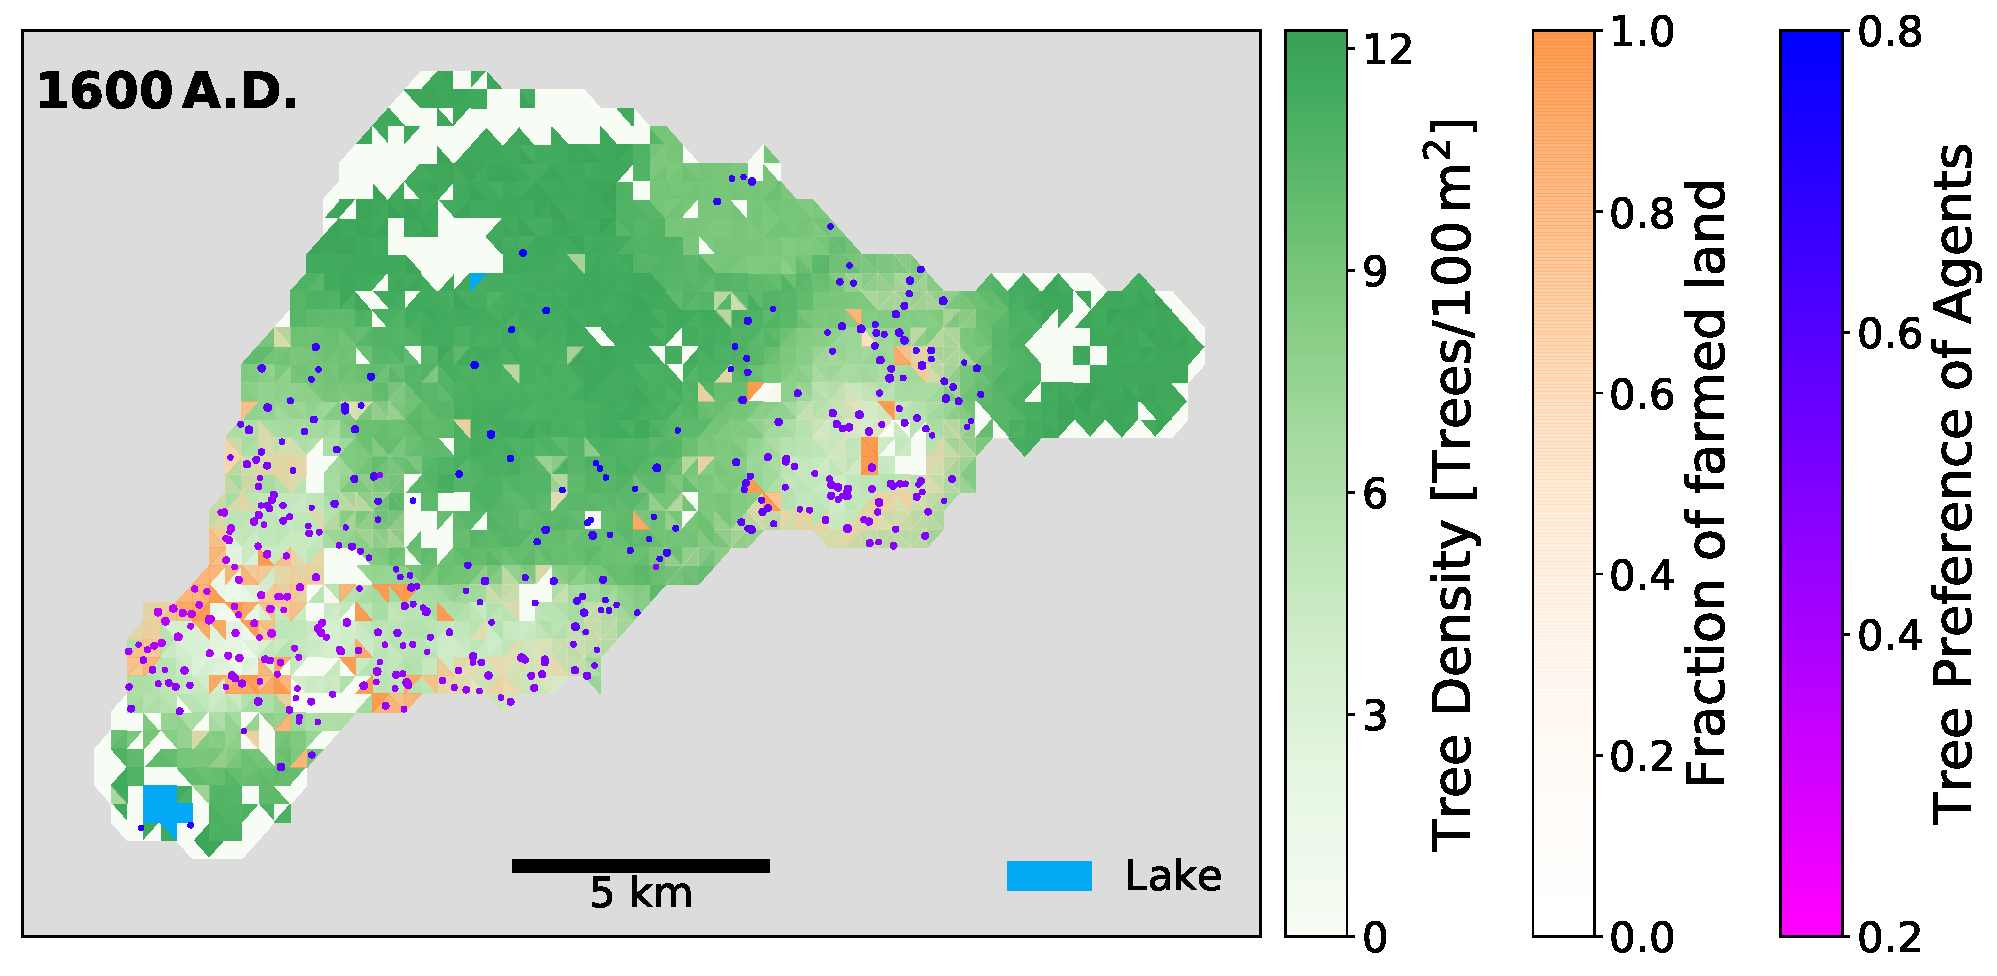
\includegraphics[width=0.7\linewidth]{images/map_time1600}
	%\captionof{figure}{Example Snapshot}
%\end{overlayarea}
\end{frame}

\begin{frame}{Create the Environment -- Discretisation}
	\centering
	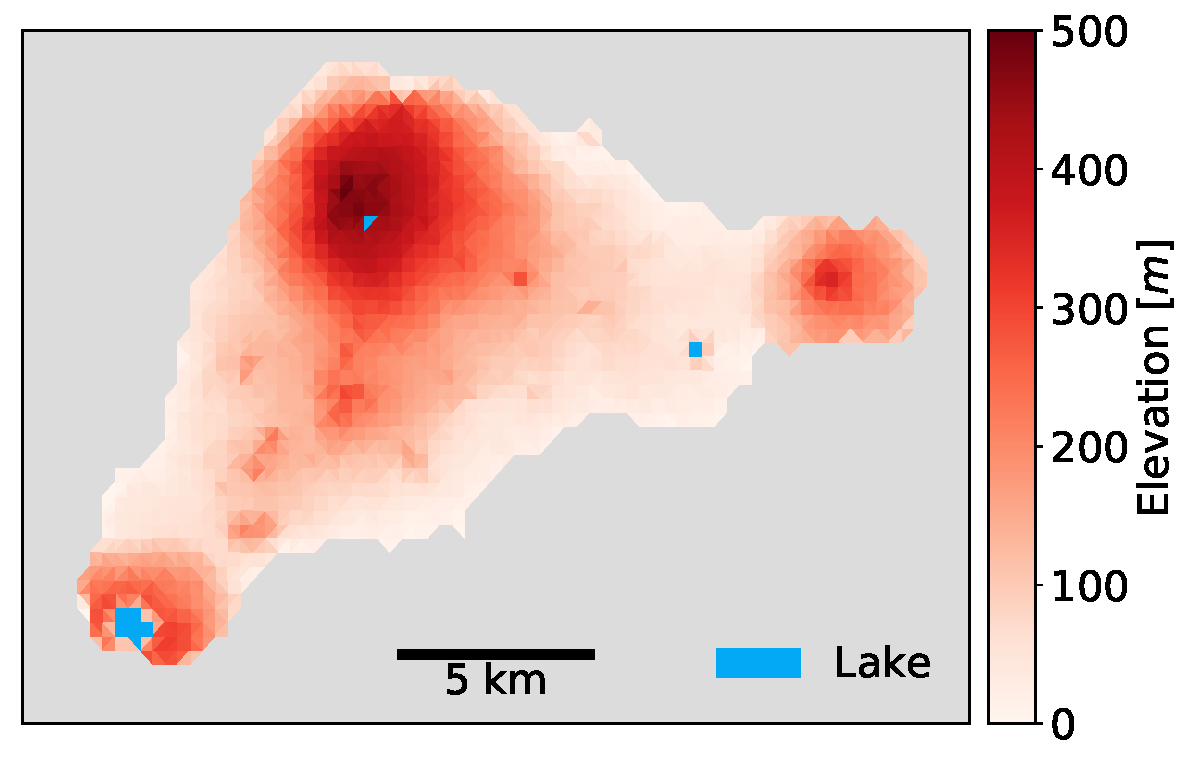
\includegraphics[width=0.7\linewidth]{Plot_elevation}


\end{frame}

\begin{frame}{Create the Environment -- Features}
\centering
\only<1>{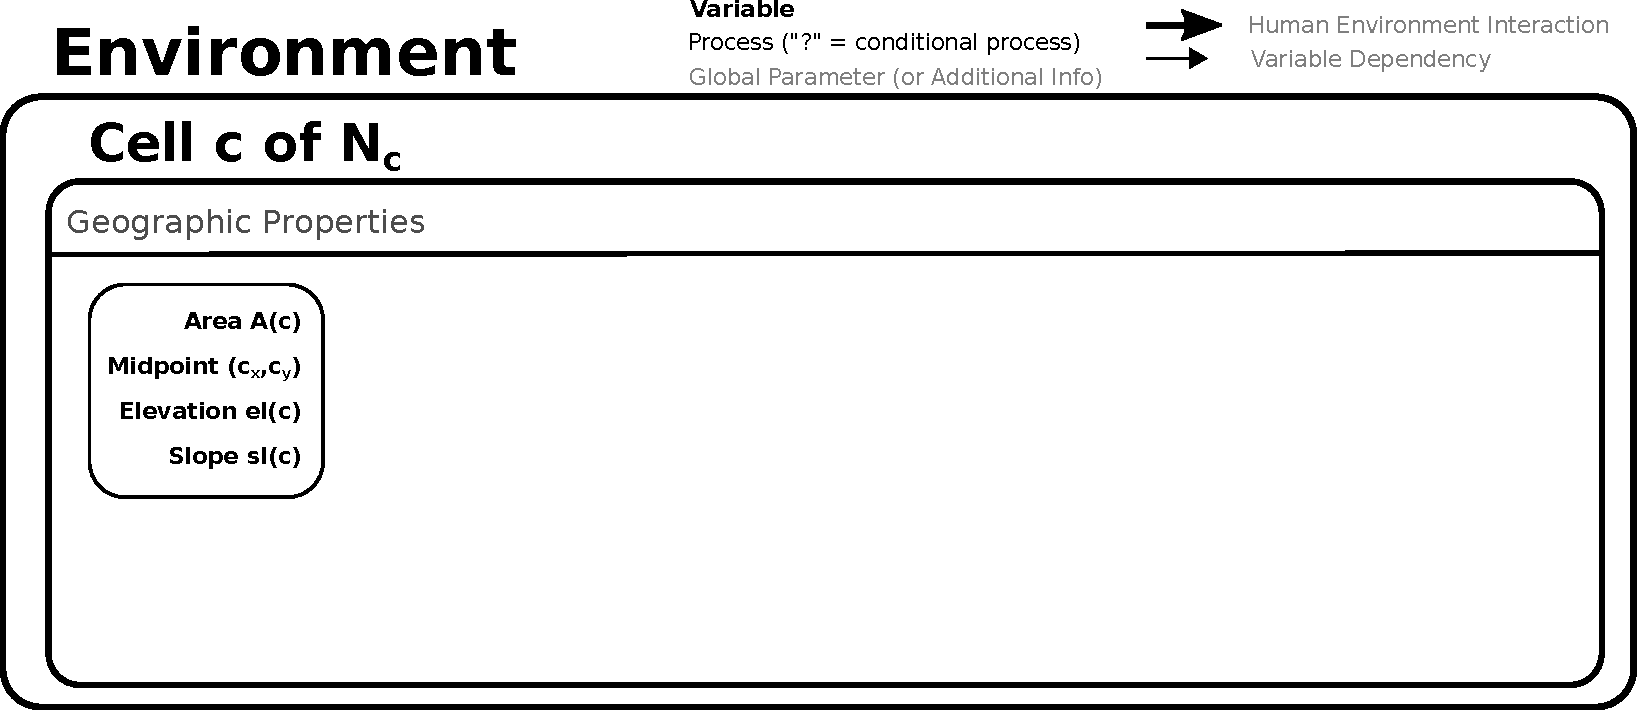
\includegraphics[width=0.7\linewidth]{SketchABM2/EnvironmentSketch_1}}
\only<2>{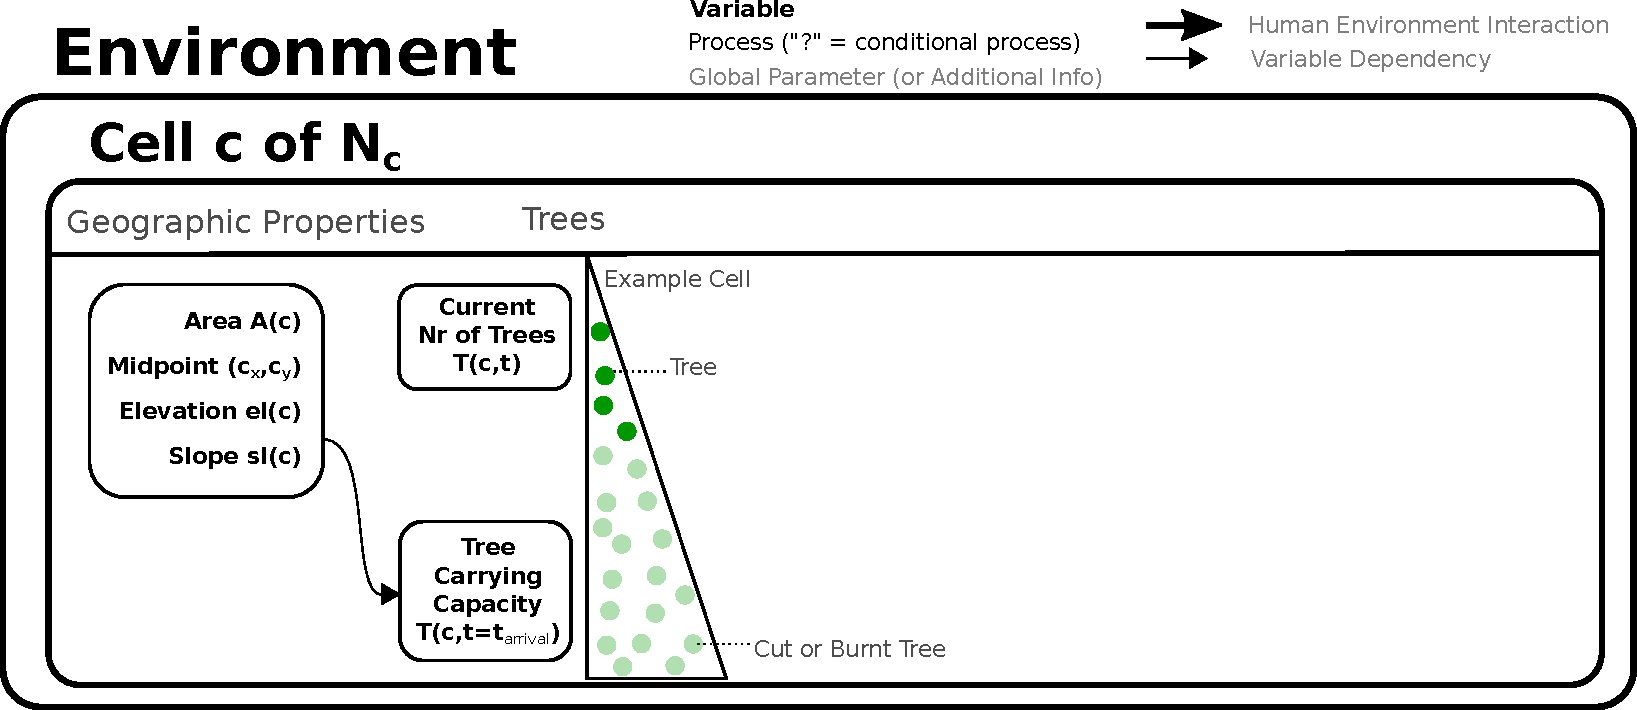
\includegraphics[width=0.7\linewidth]{SketchABM2/EnvironmentSketch_2}}
\only<3>{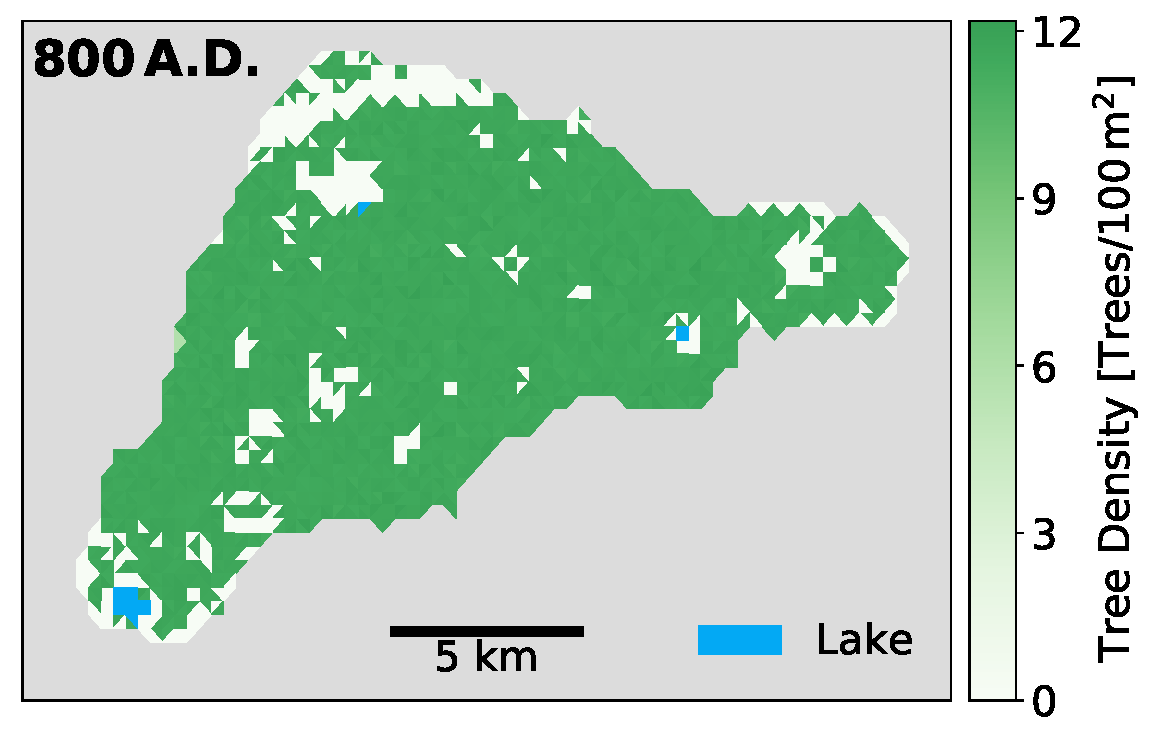
\includegraphics[width=0.7\linewidth]{map_carrCap}
\captionof{figure}{Based on \citet{Mieth2015}, \citet{Bahn2017}, \citet{Rull2020}}
}
\only<4>{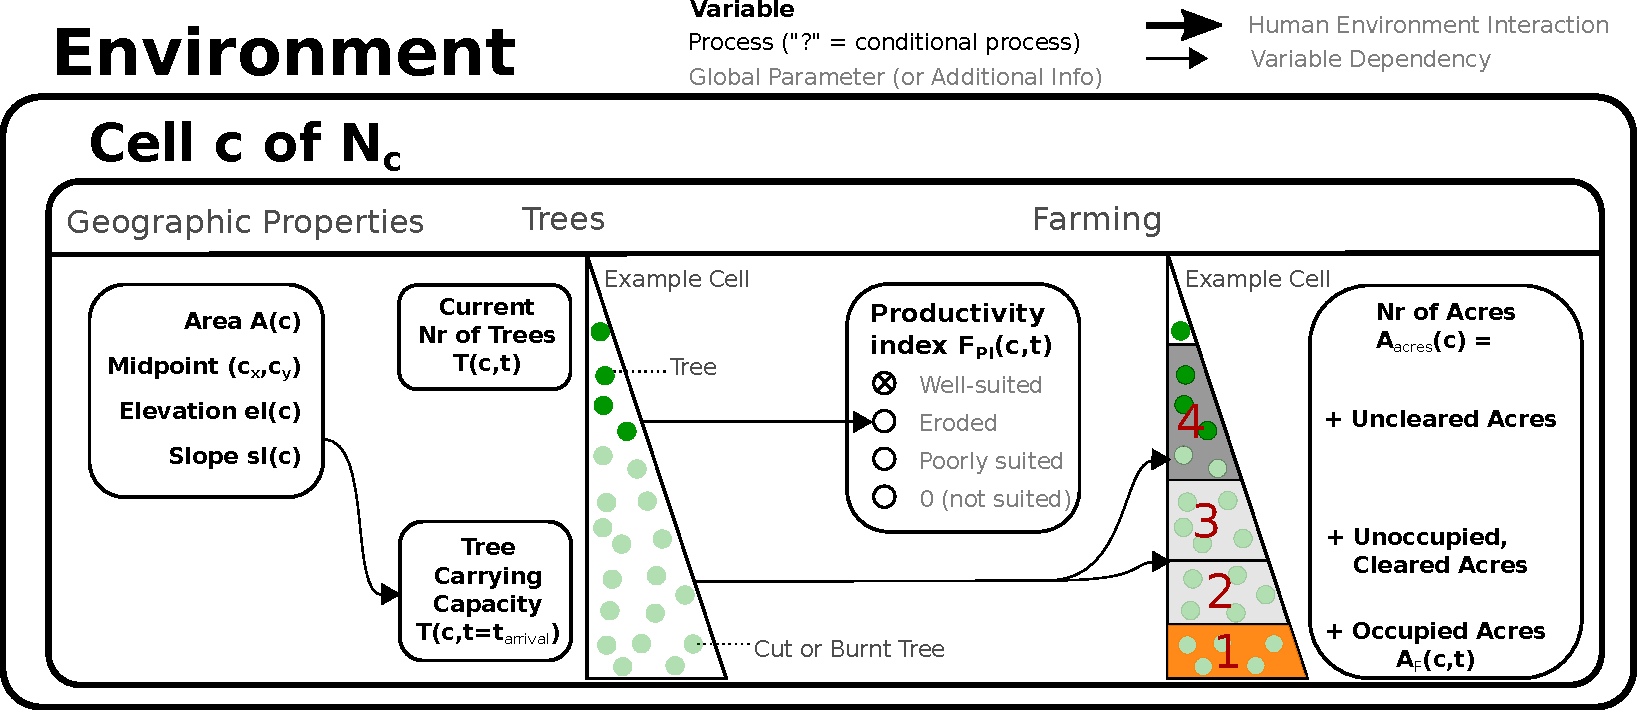
\includegraphics[width=0.7\linewidth]{SketchABM2/EnvironmentSketch_final}
	\captionof{figure}{$1\, {\rm acre} \ \hat{\approx} \ 100\, {\rm m} \, \times 40\,{\rm m}$.}}
\only<5>{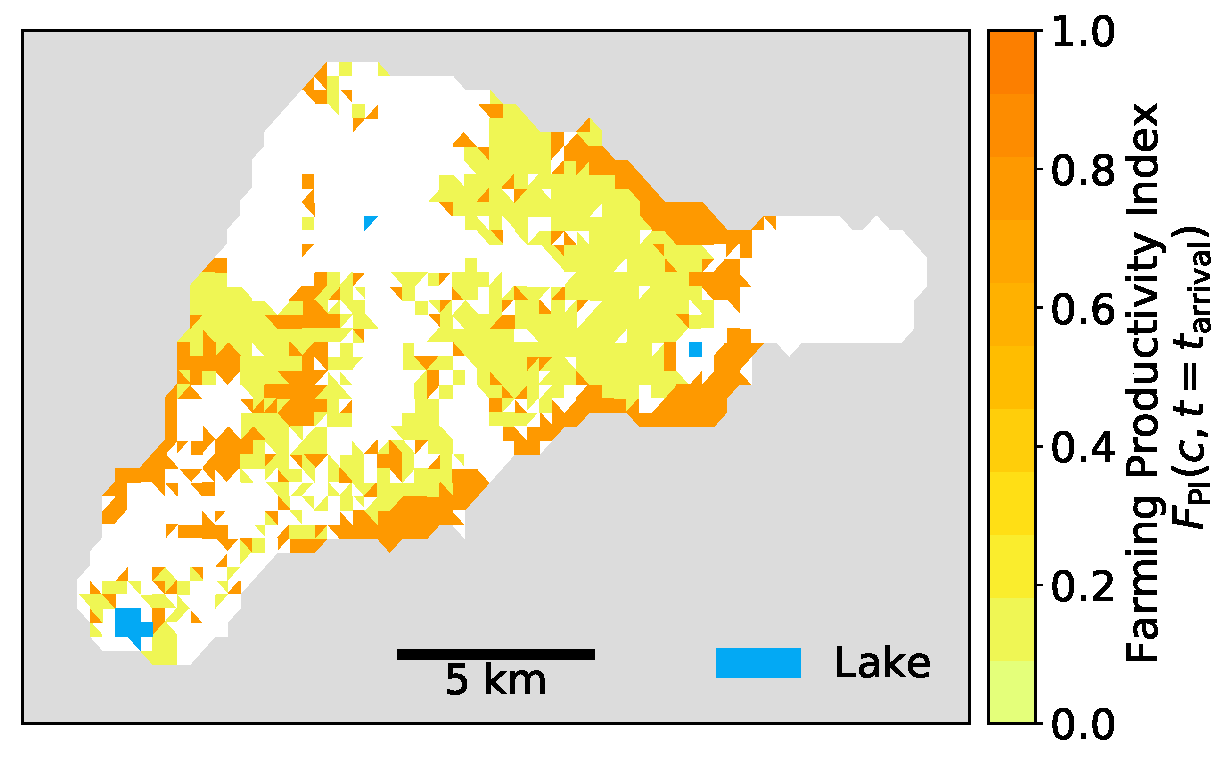
\includegraphics[width=0.7\linewidth]{Plot_F_PI_c}
	\captionof{figure}{Based on \citet{Louwagie2006}, \citet{Puleston2017}}}
\end{frame}

\begin{frame}{Agents and Interaction with Environment}
\centering
\only<1>{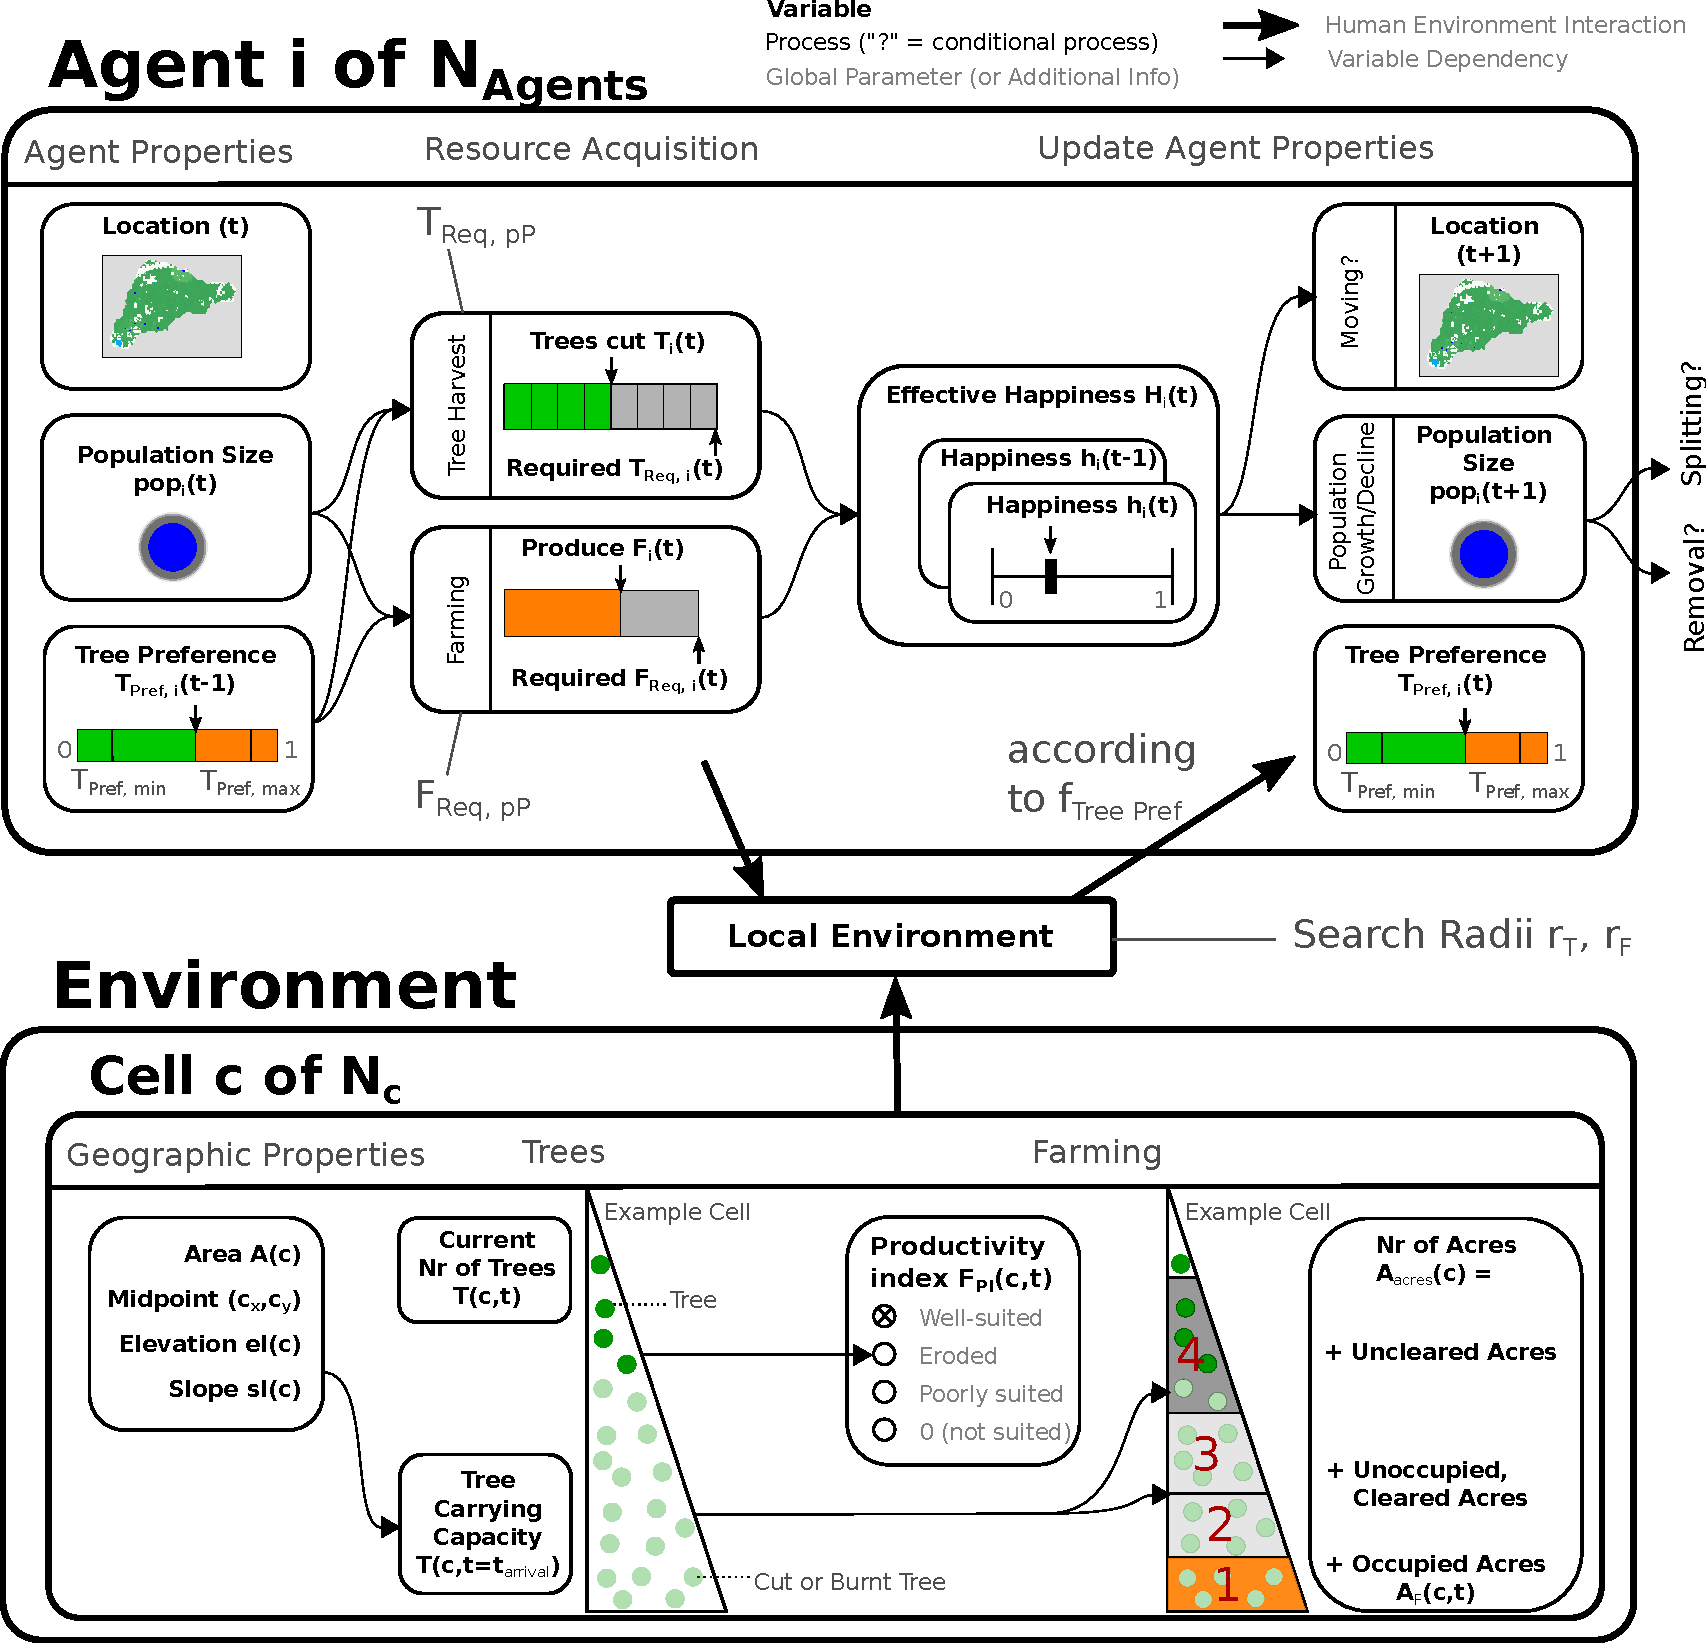
\includegraphics[width=0.55\linewidth]{SketchABM2/sketch_triangles}}
%\only<2>{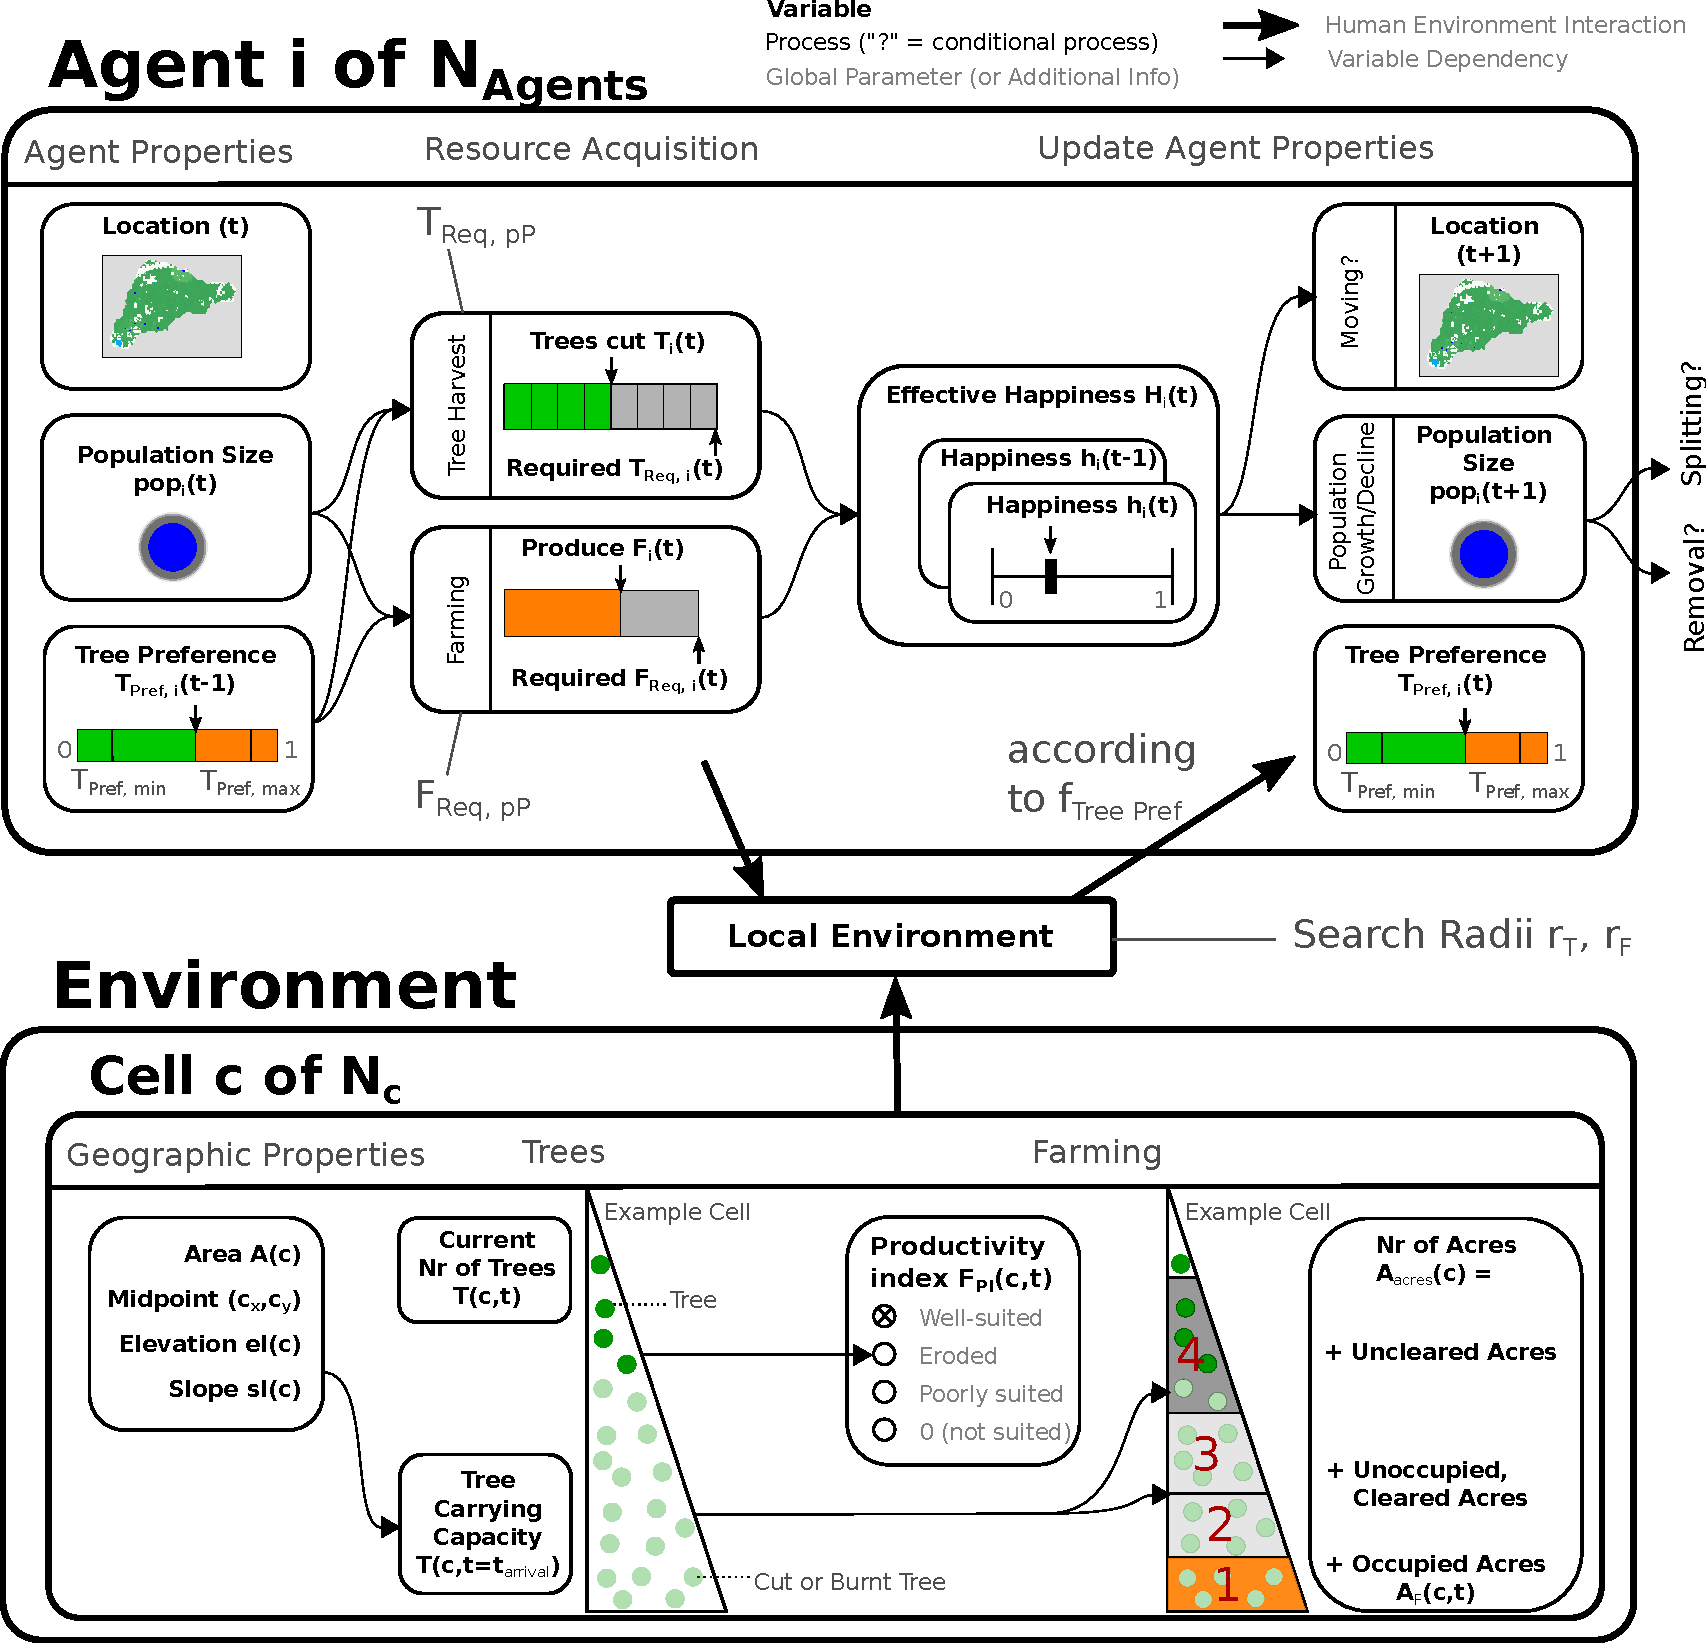
\includegraphics[width=0.85\linewidth]{SketchABM2/sketch_triangles}}
\only<2>{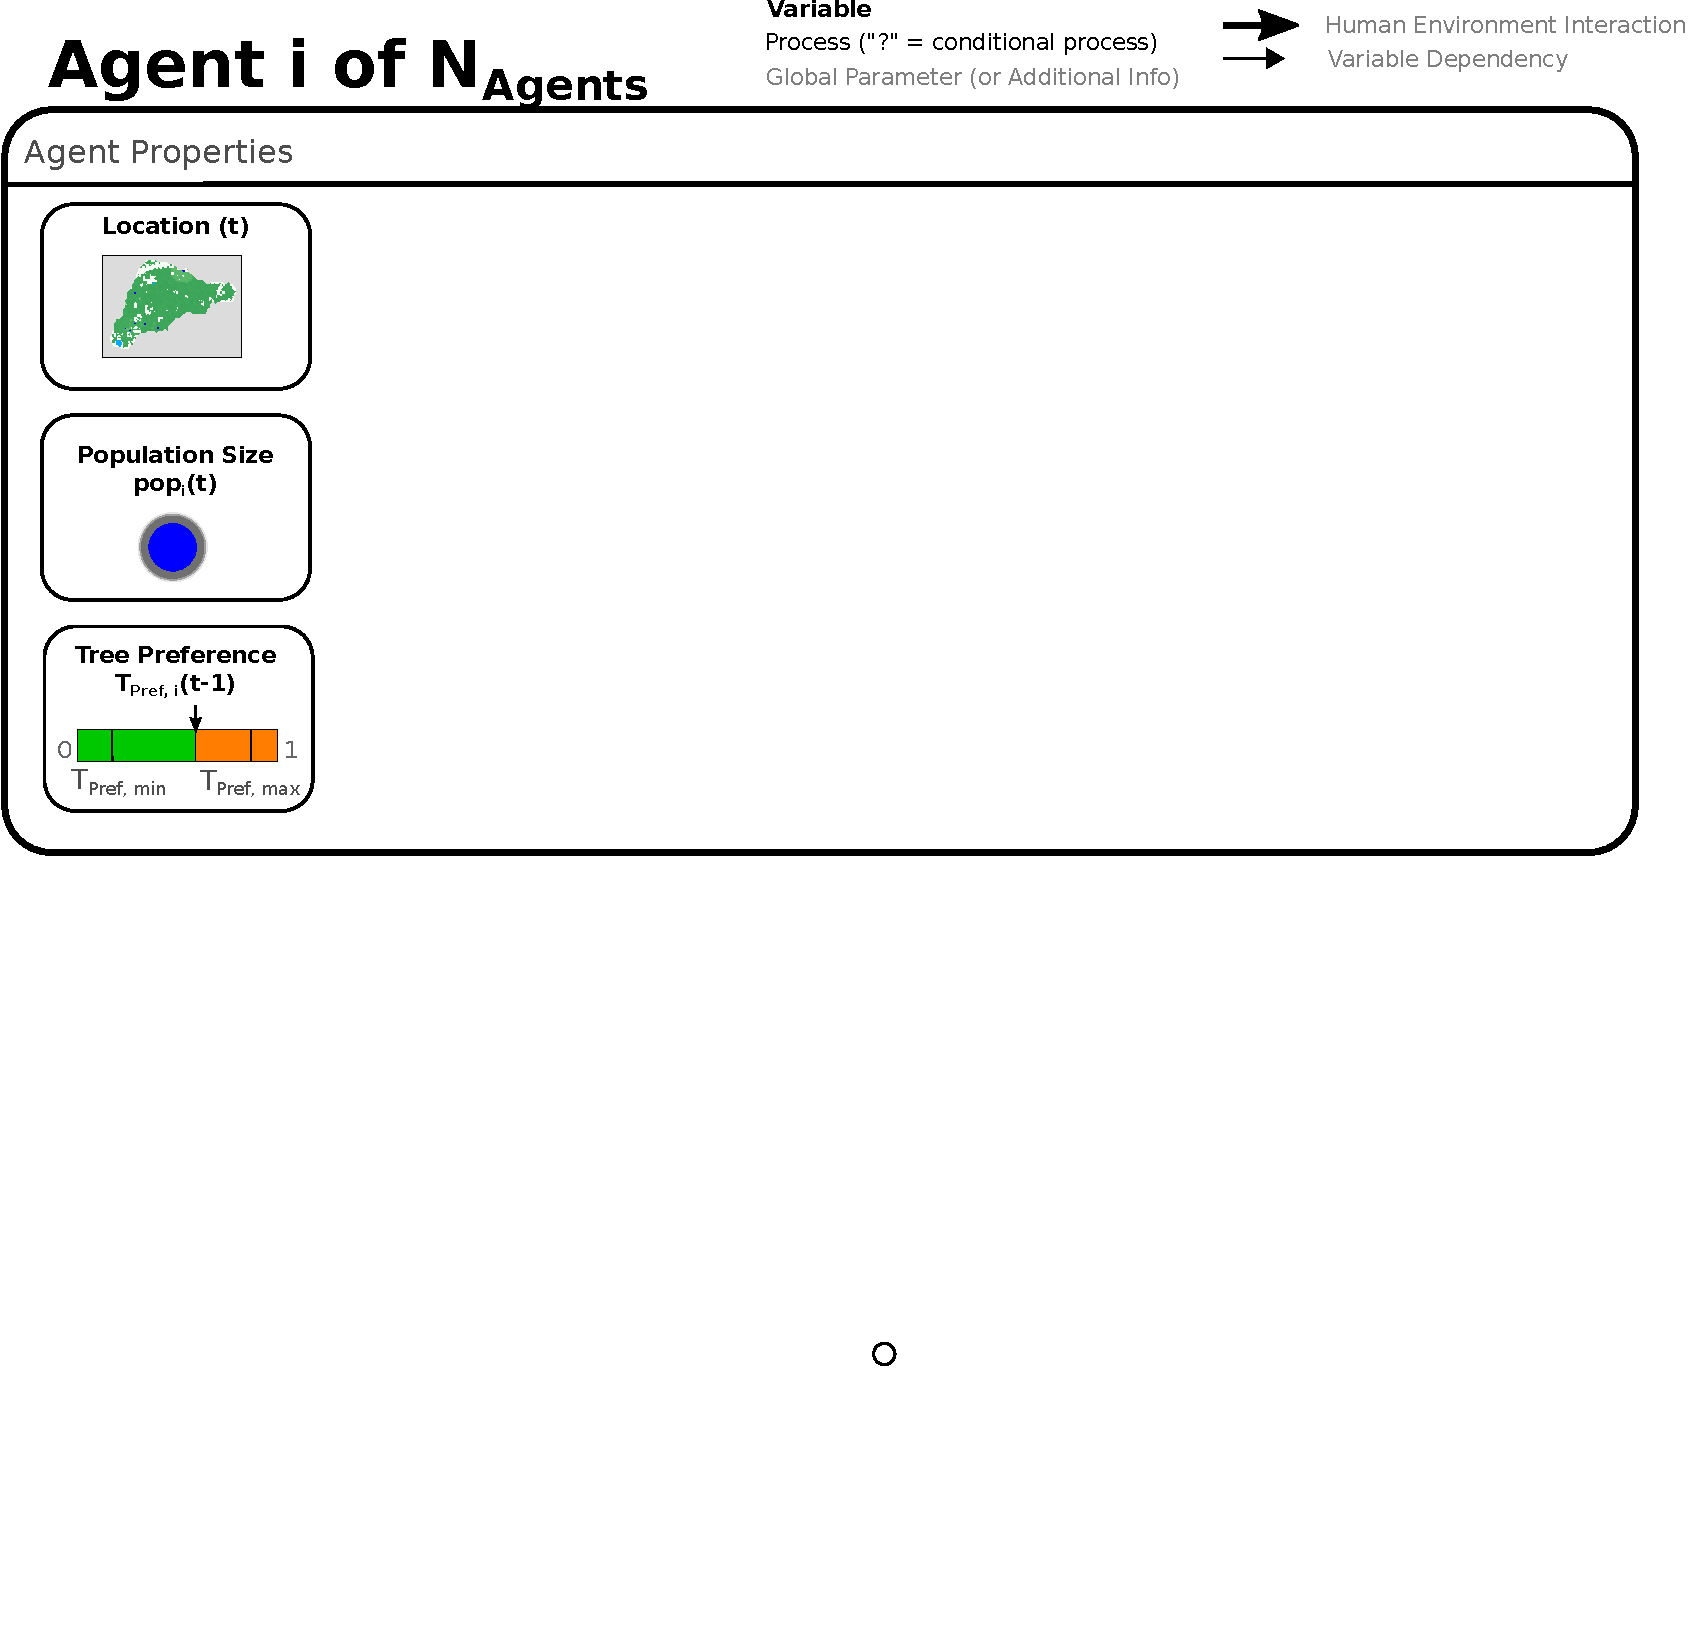
\includegraphics[width=0.85\linewidth]{SketchABM2/Agent_Props}}
\only<3>{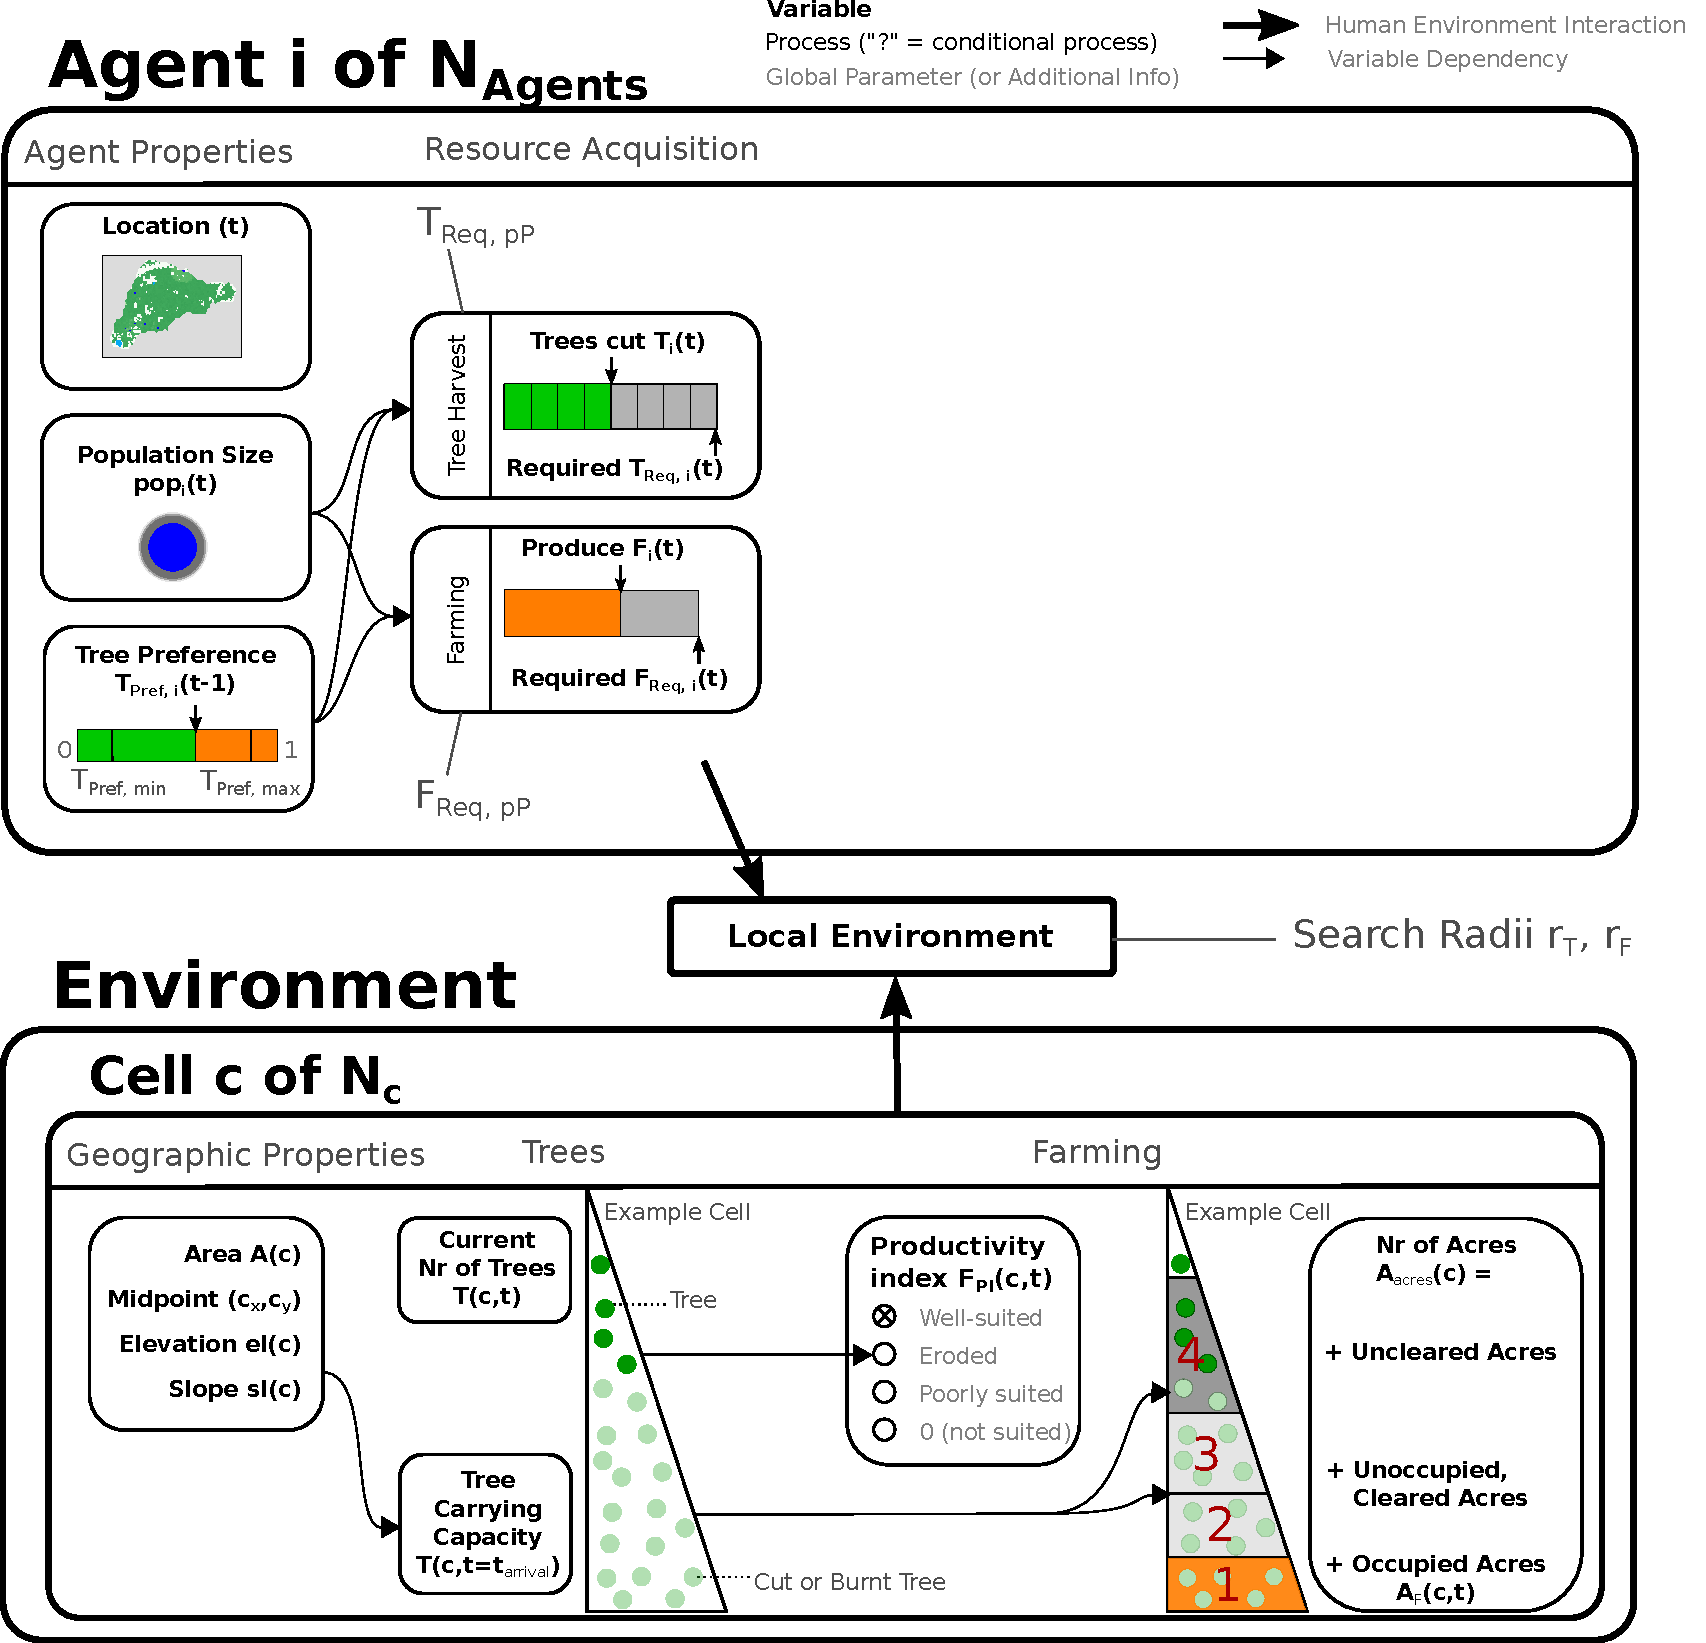
\includegraphics[width=0.85\linewidth]{SketchABM2/Agent_Harvest}}
\only<4>{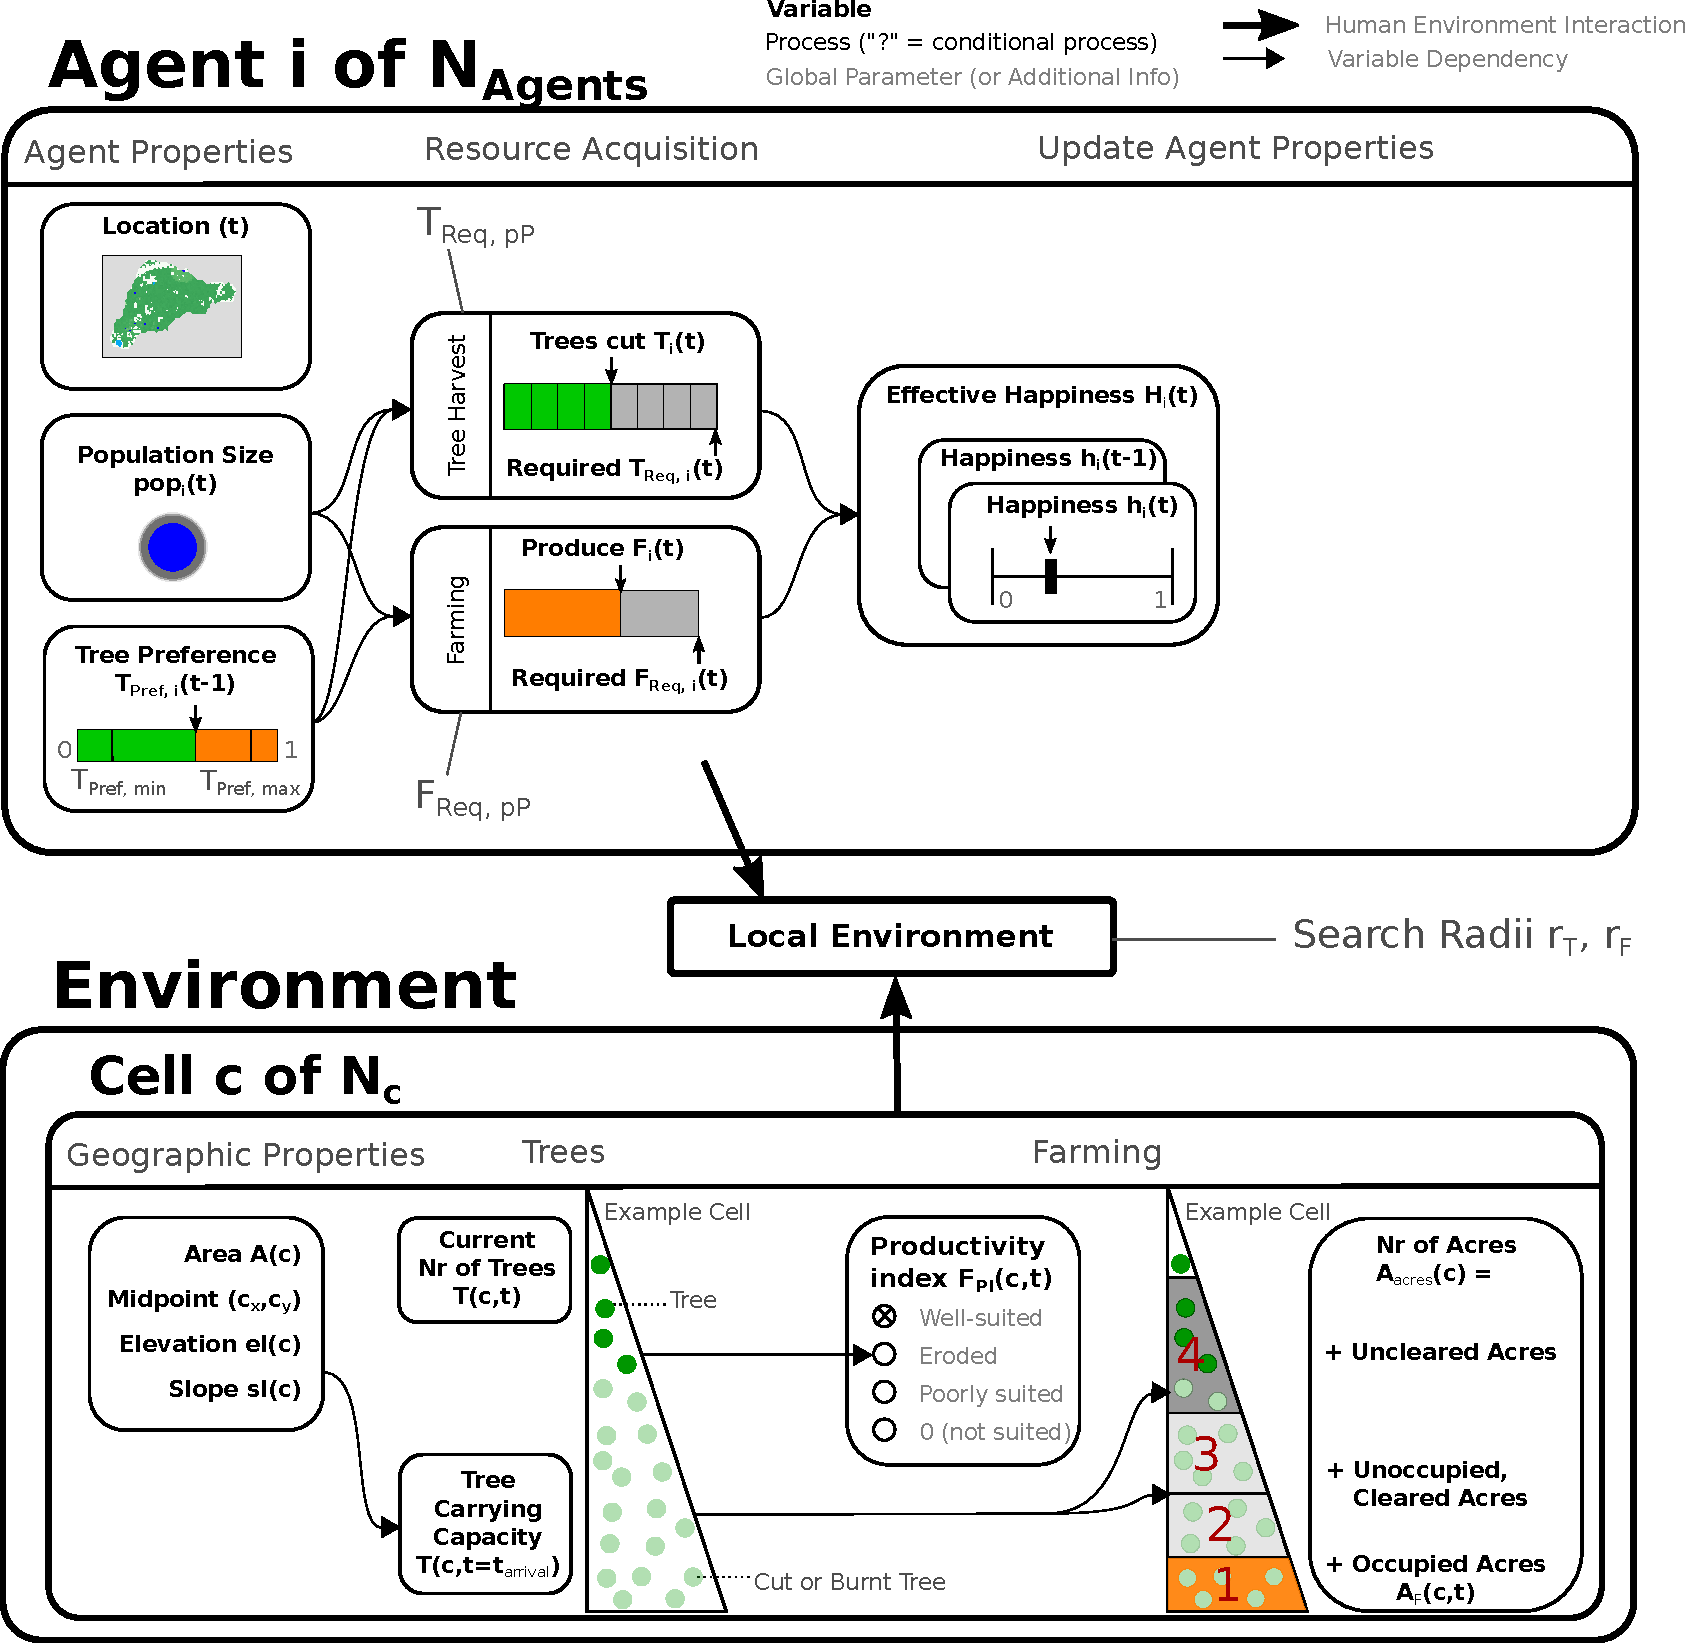
\includegraphics[width=0.85\linewidth]{SketchABM2/Agent_Update2}}
\only<5>{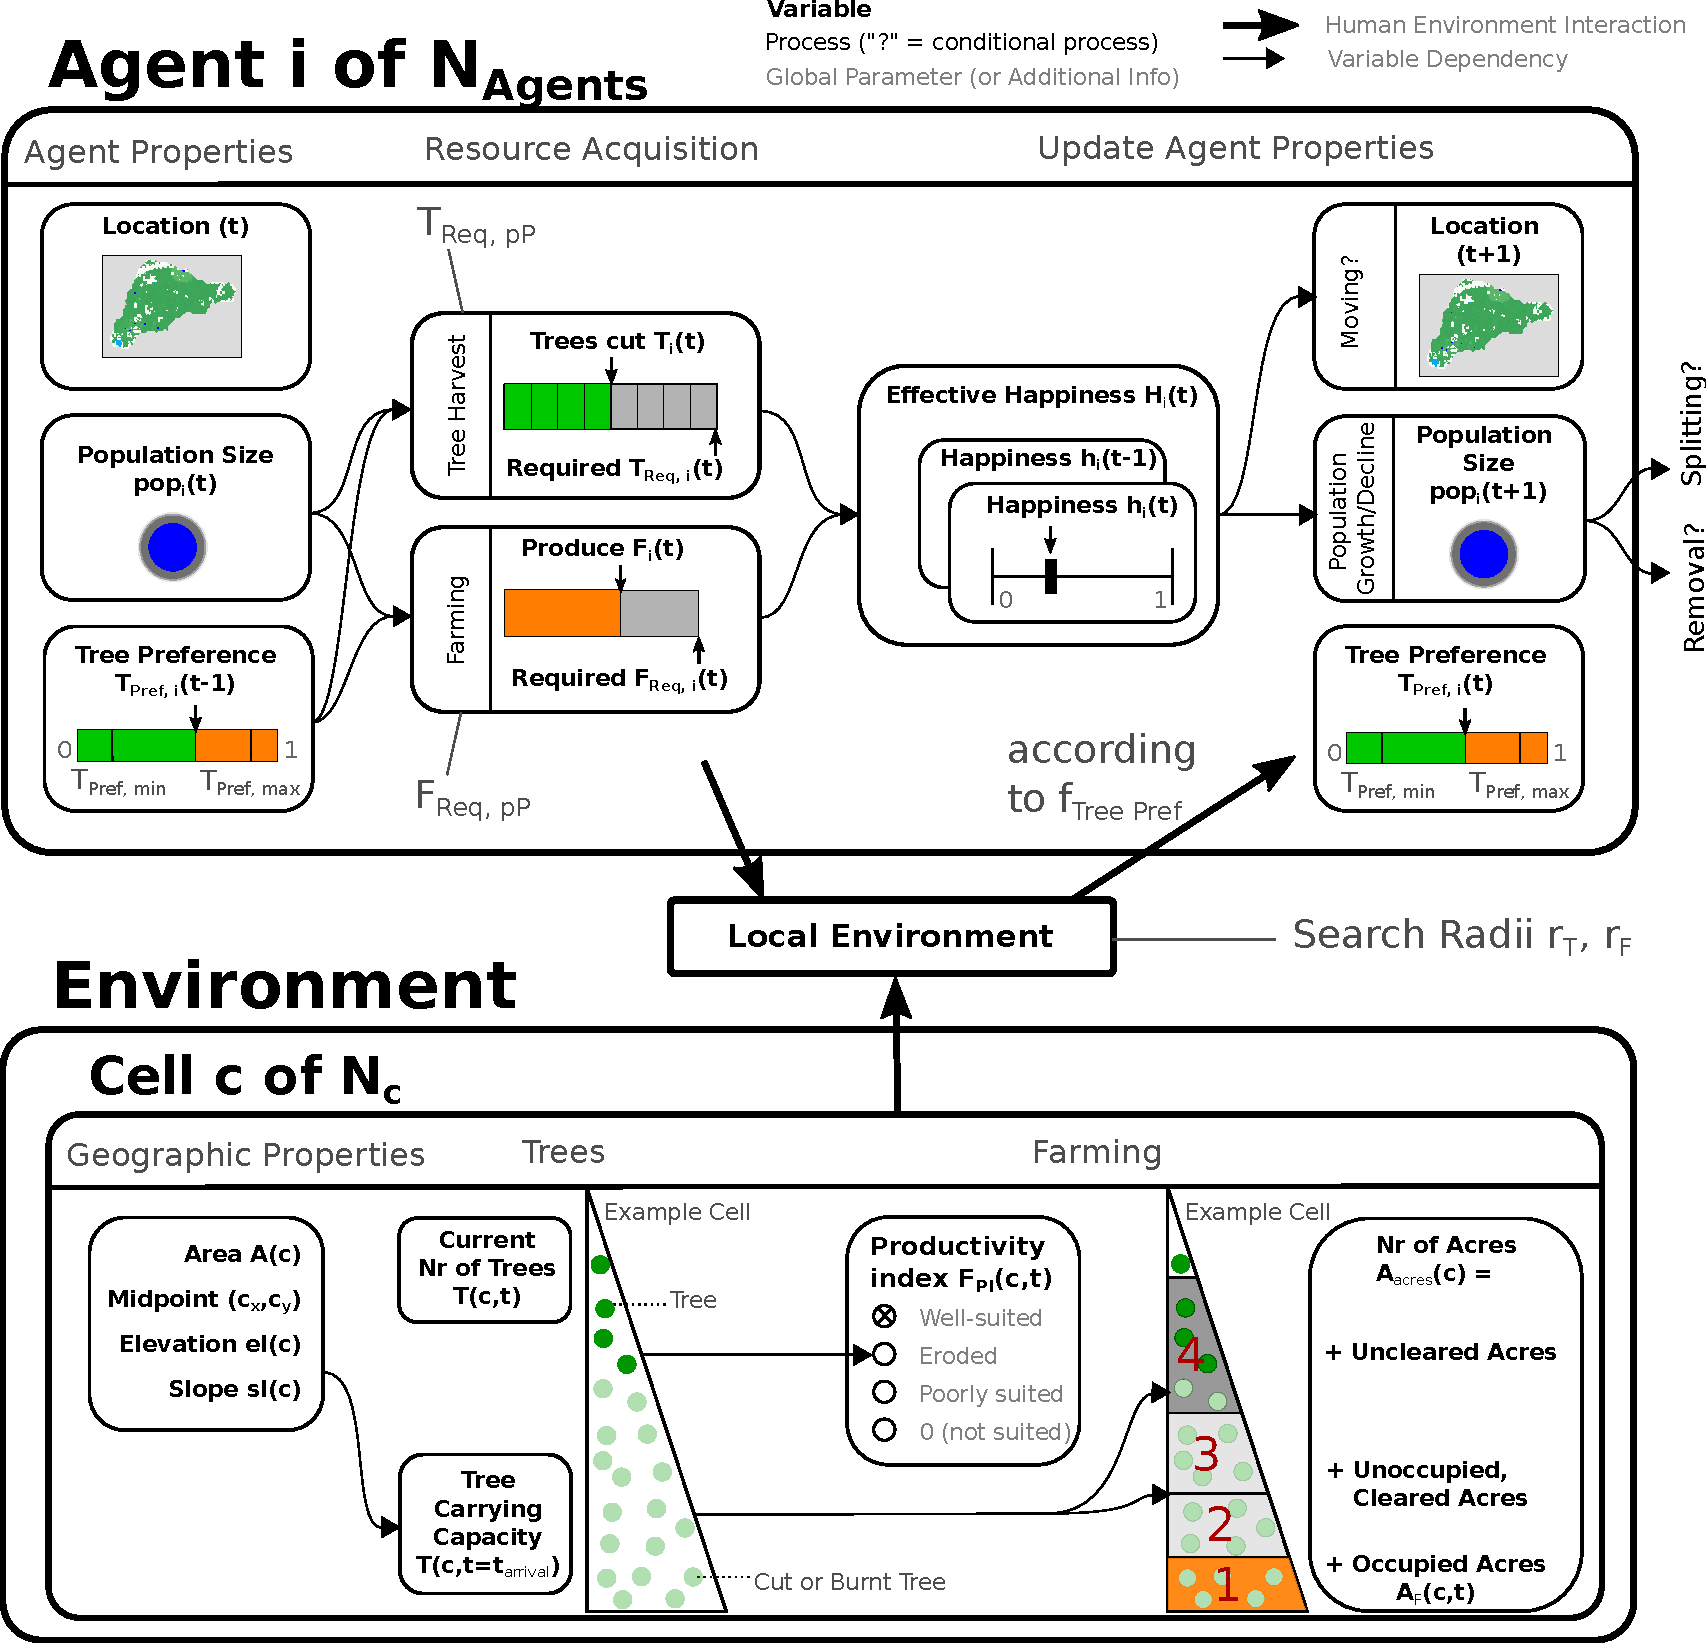
\includegraphics[width=0.85\linewidth]{SketchABM2/sketch_triangles}}
\end{frame}

%\begin{frame}
%Exceptions: Fishing.
%\end{frame}


\begin{frame}{Moving: Decision Making based on Penalties}

\begin{columns}
\begin{column}{0.2\textwidth}
	\centering
	\only<1>{
\includegraphics[height=2cm]{images/white}\captionof{figure}{\scriptsize \ \  }}
	\only<2->{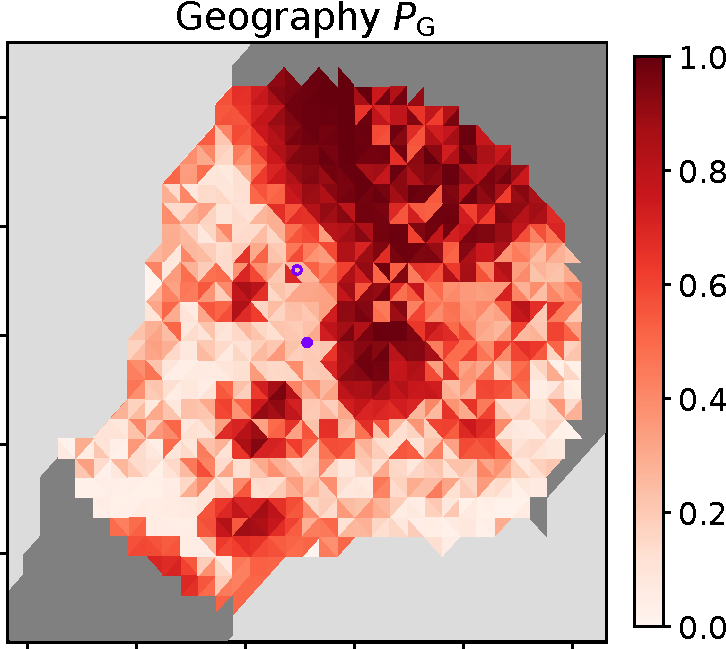
\includegraphics[height=2cm]{../../Thesis/images/Results/Standard/Penalties_AG500_t=1603_G}
	\captionof{figure}{\scriptsize Geography}}
\end{column}%\hfill
\begin{column}{0.2\textwidth}
	\centering
	\only<3->{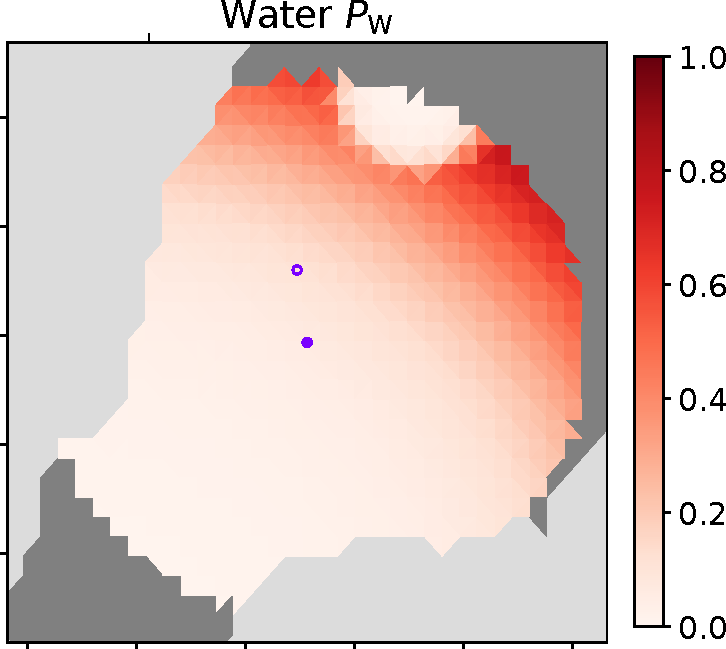
\includegraphics[height=2cm]{../../Thesis/images/Results/Standard/Penalties_AG500_t=1603_W}
	\captionof{figure}{\scriptsize Water}}
\end{column} 
\begin{column}{0.2\textwidth}
\centering
\only<4->{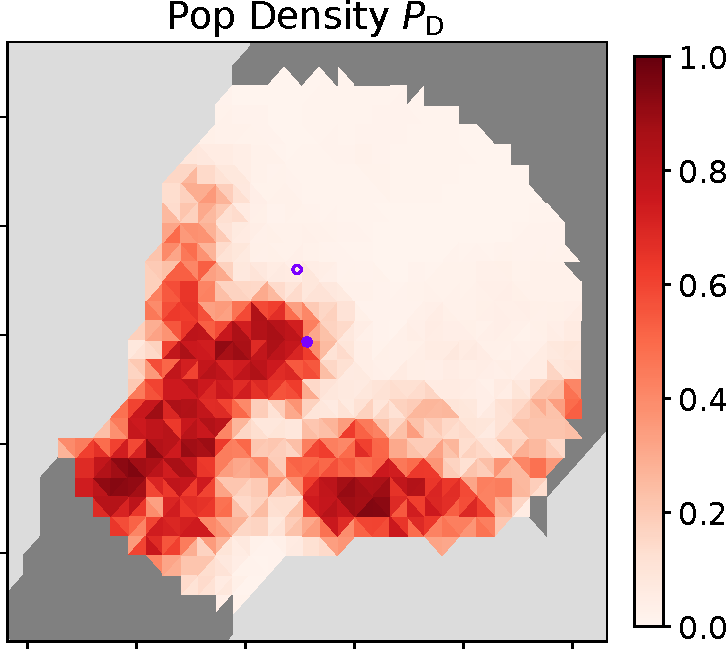
\includegraphics[height=2cm]{../../Thesis/images/Results/Standard/Penalties_AG500_t=1603_D}
	\captionof{figure}{\scriptsize Pop.\ Density}}
\end{column}
\begin{column}{0.2\textwidth}
\centering
\only<5->{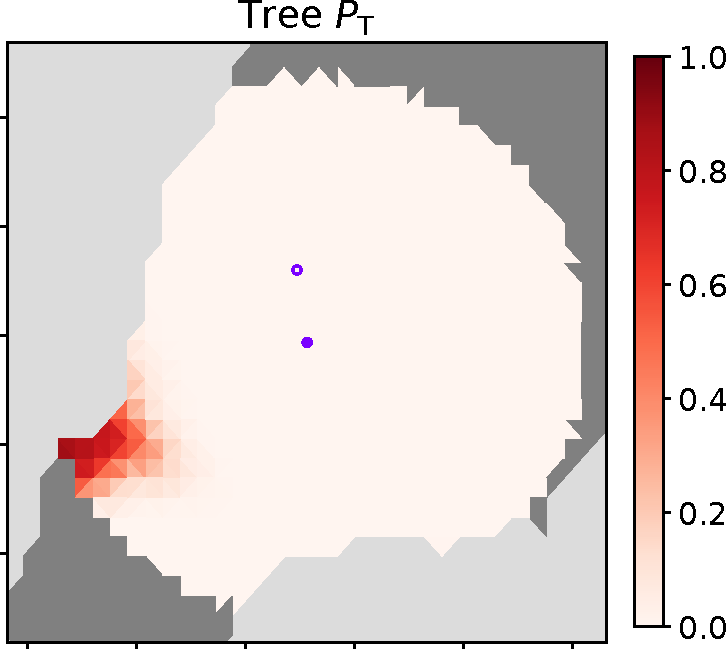
\includegraphics[height=2cm]{../../Thesis/images/Results/Standard/Penalties_AG500_t=1603_T}
	\captionof{figure}{\scriptsize Trees}}
\end{column}
\begin{column}{0.19\textwidth}
\centering
\only<6->{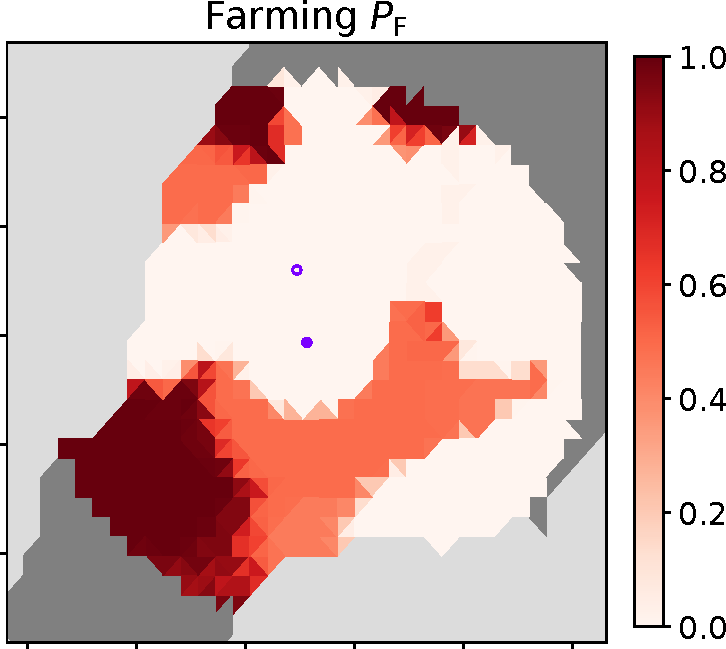
\includegraphics[height=2cm]{../../Thesis/images/Results/Standard/Penalties_AG500_t=1603_F}
	\captionof{figure}{\scriptsize Farming Sites}}
\end{column}
\end{columns}

\vfill
\centering
\begin{columns}
	\begin{column}{0.35\textwidth}
		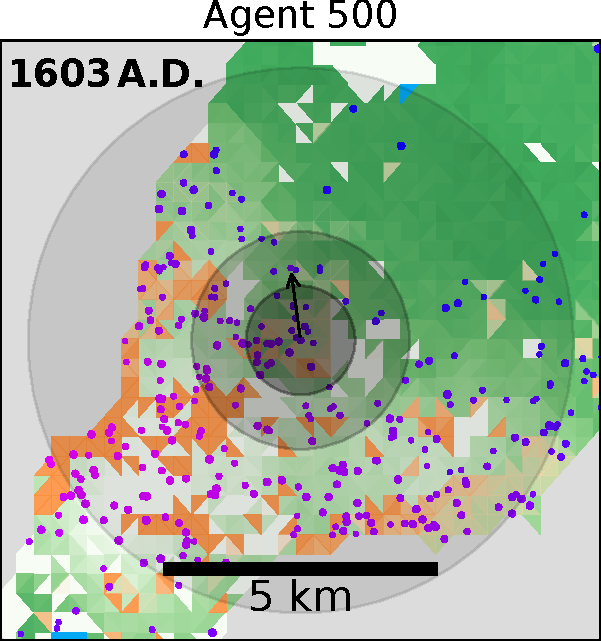
\includegraphics[height=4.5cm]{../../Thesis/images/Results/Standard/Penalties_AG500_t=1603_Situation}
	\end{column}
	\begin{column}[t]{0.25\textwidth}
	 	\only<2>{\textbf{Avoid cells...\\ ...
	  	with large elevation and large slope}}%
  		\only<3>{\textbf{Avoid cells...\\ ...
  				far from a (big) freshwater source   }}%
  		\only<4>{\textbf{Avoid cells...\\ ...
  				in regions with large population density}}%	
 			\only<5>{\textbf{Avoid cells...\\...
 					with few trees nearby  }}%
				\only<6>{\textbf{Avoid cells... \\ ...
						with few (well-suited) available farming sites nearby}}%
  		\only<7>{\textbf{\begin{center} {\Huge$\Downarrow$} \end{center} \ra \quad Total\quad \ra }}
  	
	\end{column}
	\begin{column}{0.35\textwidth}
		\only<2>{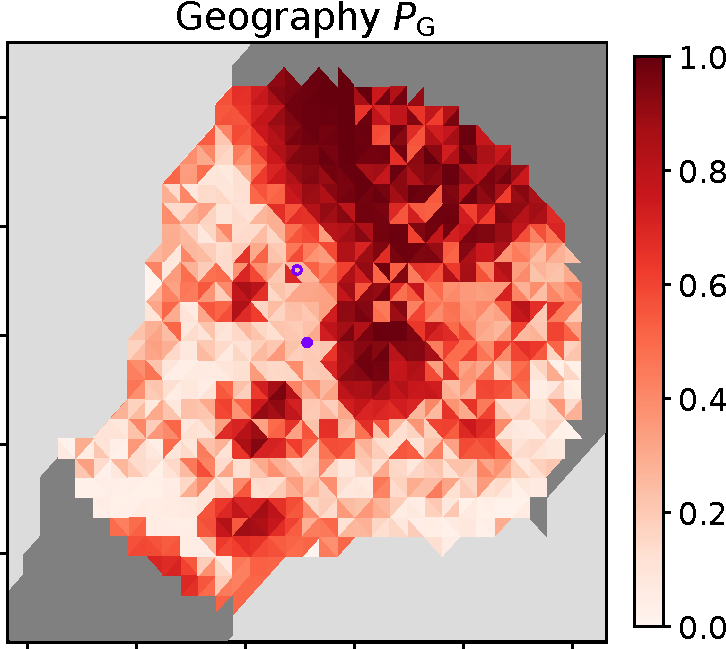
\includegraphics[height=4.5cm]{../../Thesis/images/Results/Standard/Penalties_AG500_t=1603_G}}%
		\only<3>{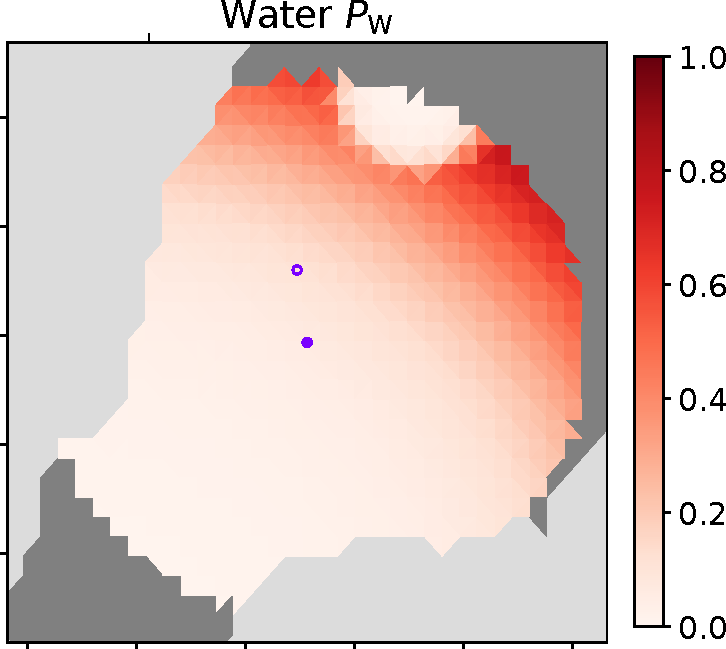
\includegraphics[height=4.5cm]{../../Thesis/images/Results/Standard/Penalties_AG500_t=1603_W}}%
		\only<4>{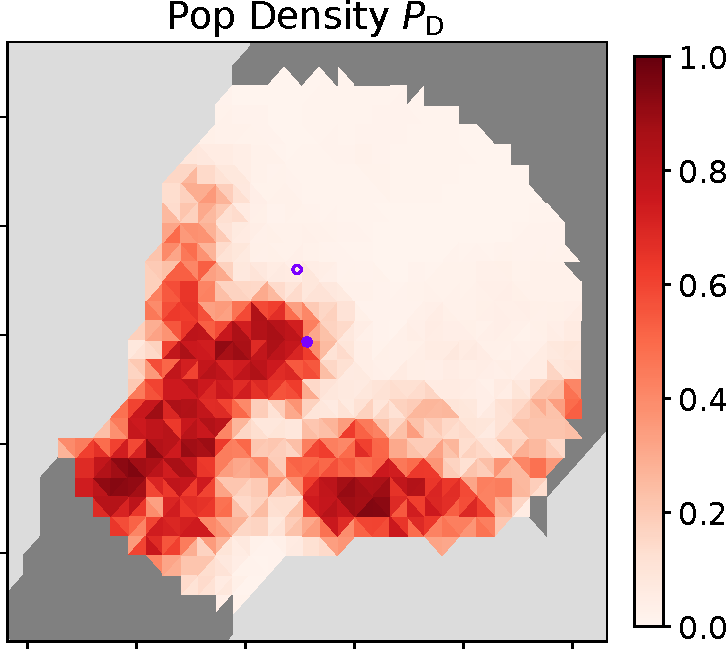
\includegraphics[height=4.5cm]{../../Thesis/images/Results/Standard/Penalties_AG500_t=1603_D}}%	
		\only<5>{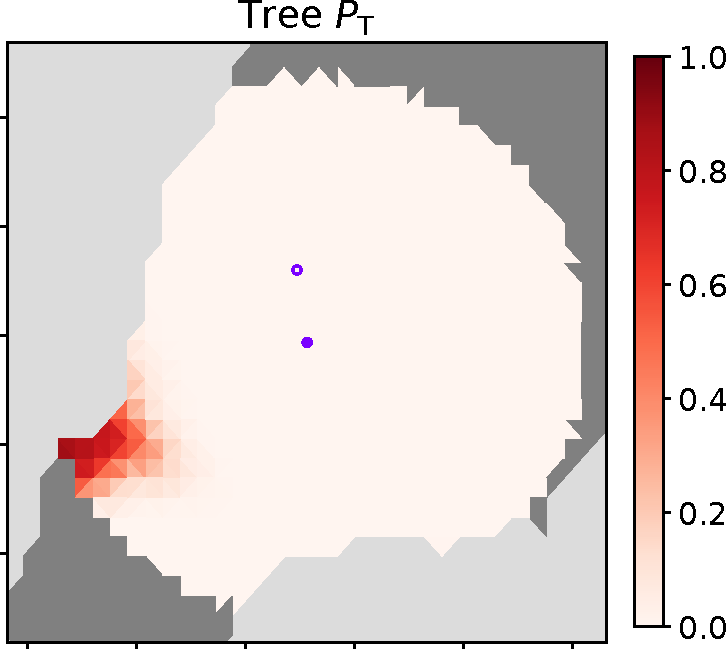
\includegraphics[height=4.5cm]{../../Thesis/images/Results/Standard/Penalties_AG500_t=1603_T}}%	
		\only<6>{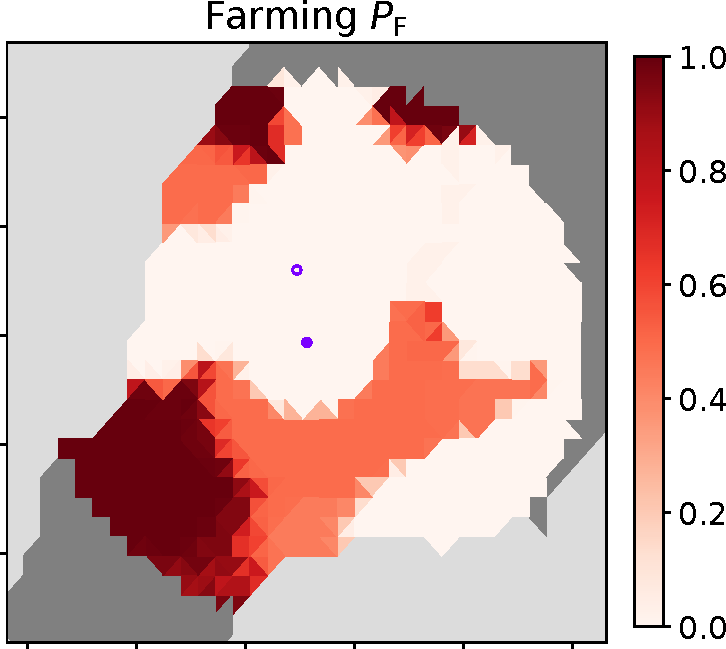
\includegraphics[height=4.5cm]{../../Thesis/images/Results/Standard/Penalties_AG500_t=1603_F}}%
		\only<7>{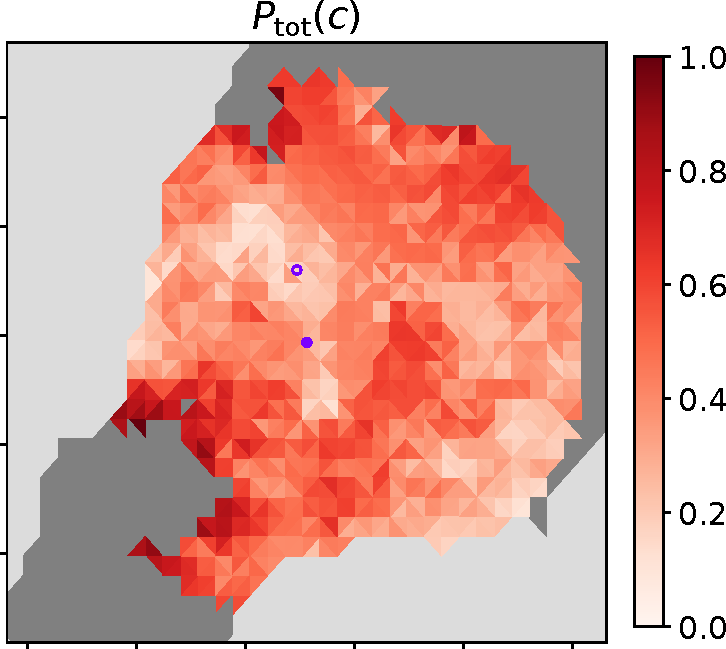
\includegraphics[height=4.5cm]{../../Thesis/images/Results/Standard/Penalties_AG500_t=1603_tot}}
	\end{column}
\end{columns}
%

\end{frame}


\begin{frame}{The Full Model}
\begin{columns}
	\column[T]{0.69\textwidth}
		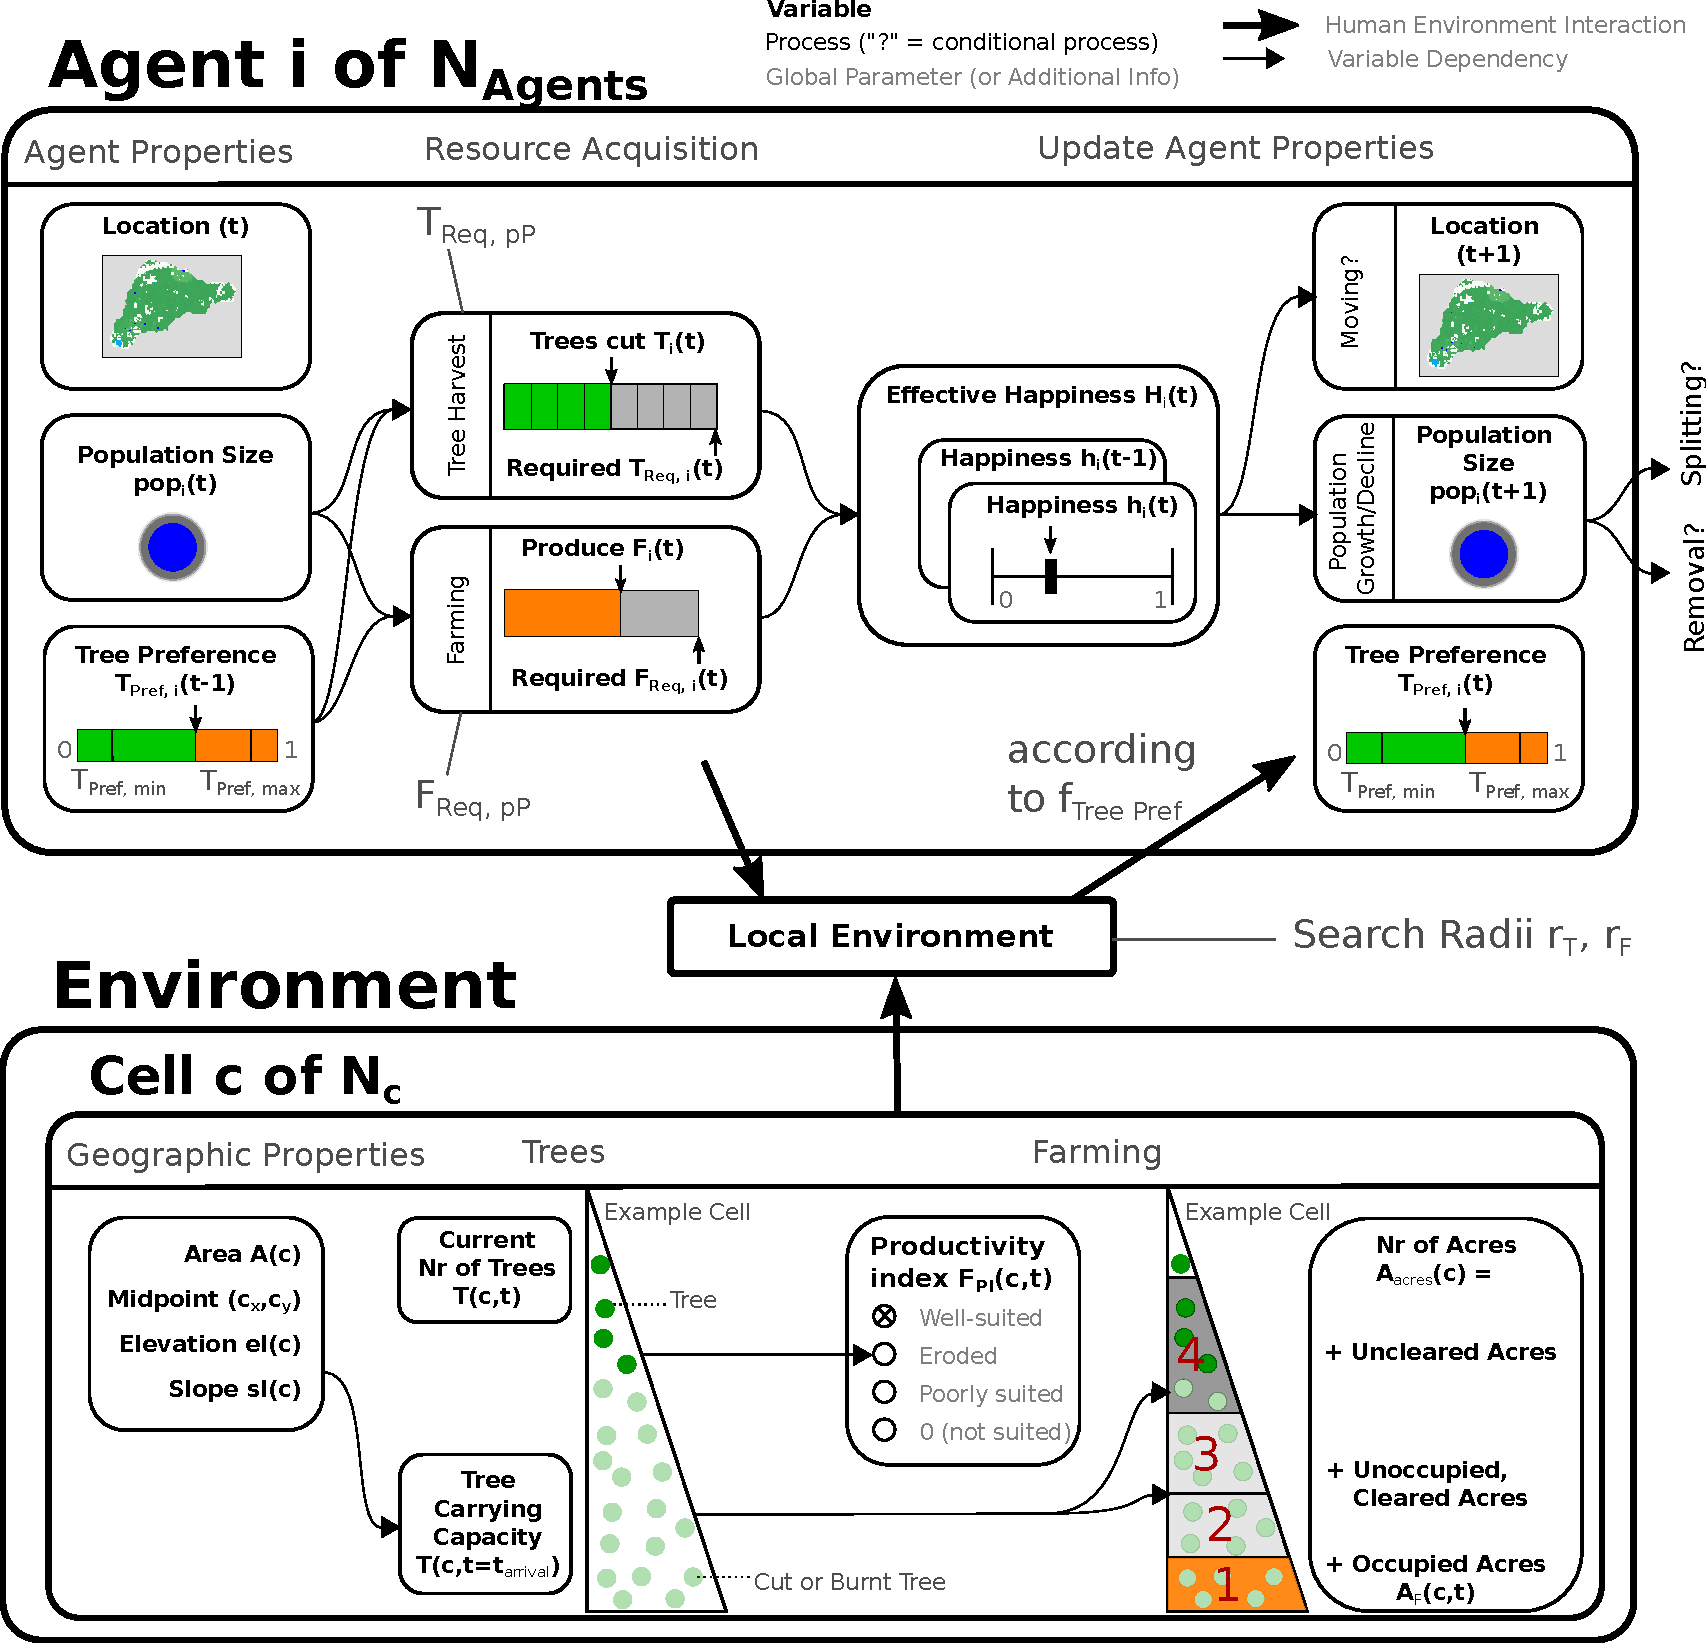
\includegraphics[height=0.85\textheight]{SketchABM2/sketch_triangles}
	\column[T]{0.29\textwidth}
		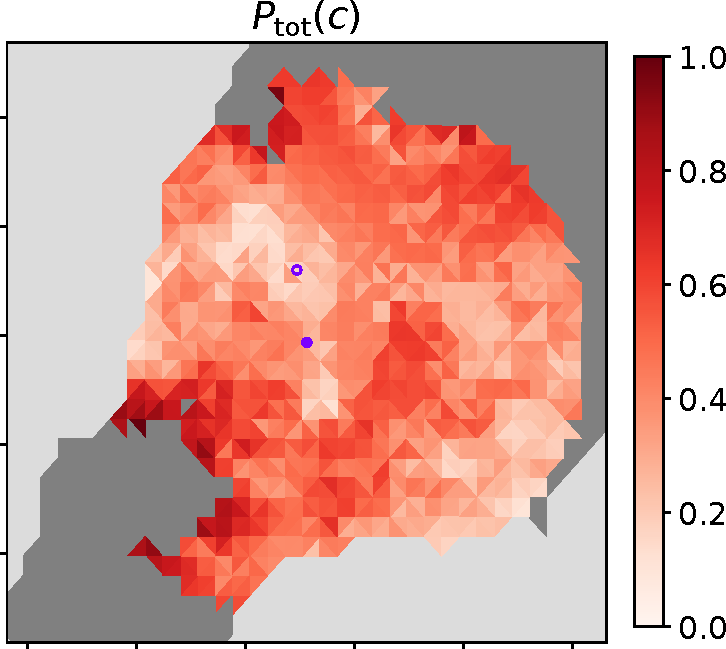
\includegraphics[height=3.5cm]{../../Thesis/images/Results/Standard/Penalties_AG500_t=1603_tot}
\end{columns}
\end{frame}
	


